\documentclass[11pt,a4paper]{article}

\usepackage{amsfonts,amssymb,amsmath}
\usepackage[margin=1in]{geometry}
\usepackage[none]{hyphenat}
\usepackage{graphicx}
\usepackage{fancyhdr}
\usepackage{float}
\usepackage{color}
\usepackage{xcolor}
\usepackage{tikz}
% Straight quotes in verbatim, so that code copied from the notes runs.
\usepackage{upquote}
\usepackage[nottoc,notlot,notlof]{tocbibind}

\usetikzlibrary{arrows.meta,shapes,positioning}

\parindent 0ex
% hyphenat[none] forbids hyphenation, so give TeX room to stretch a line
% instead of letting it run into the margin.
\setlength{\emergencystretch}{3em}
\setlength{\parskip}{0.55\baselineskip}
\setlength{\abovedisplayskip}{0.5\baselineskip}
\setlength{\belowdisplayskip}{0.5\baselineskip}
\setlength{\abovedisplayshortskip}{0.25\baselineskip}
\setlength{\belowdisplayshortskip}{0.25\baselineskip}
\numberwithin{equation}{section}

\pagestyle{fancy}
\fancyfoot[C]{\thepage}
\fancyhead{}
\fancyhead[R]{\rightmark}
\renewcommand{\headrulewidth}{0pt}

% Upright operator names.
\DeclareMathOperator{\tr}{tr}
\DeclareMathOperator{\rank}{rank}
\DeclareMathOperator{\sgn}{sgn}
\DeclareMathOperator{\Real}{Re}
\DeclareMathOperator{\Imag}{Im}

% Theorem environments.
\usepackage{amsthm}
\theoremstyle{definition}
% One shared counter running section.subsection.n, as in the other courses here.
\newtheorem{thm}{Theorem}[subsection]
\newtheorem{defn}[thm]{Definition}
\newtheorem{exa}[thm]{Example}
\newtheorem{prop}[thm]{Proposition}
\newtheorem{coro}[thm]{Corollary}
\newtheorem{lem}[thm]{Lemma}
% An ``In software'' panel: the Python commands, the output they print, and how to read
% it. The web build gives these their own colour (build.py tags the type from
% the label, and ``Software'' is tested before every other label).
\newtheorem{software}[thm]{Software}
\newtheorem*{note}{Note}
\newtheorem*{remark}{Remark}
\newtheorem{problemx}{Problem}[subsection]
\newenvironment{problem}{\begin{problemx}}{\end{problemx}}
\newenvironment{solution}
  {\renewcommand{\qedsymbol}{}\begin{proof}[\textit{Solution}.]}
  {\end{proof}}
\usepackage{enumitem}
% A heading that is legal inside a theorem body, a list or a float, where
% \subsubsection is not. Same weight as \subsubsection* so the two read alike.
\newcommand{\subhead}[1]{%
  \par\medskip\noindent\textbf{#1}\par\nobreak\smallskip}

\begin{document}
% Title page depersonalised for the web, as with every other course here. The
% identity kept below is the duality theorem of linear programming, the result
% on which most of the course's theory rests.
\begin{titlepage}
\thispagestyle{empty}
\begin{center}
\vspace*{3cm}
{\Huge\bfseries Operations Research}\\[1.2cm]
{\large Lecture Notes}\\[2.5cm]
\line(1,0){300}\\[1.5cm]
$$\max\{c^{\mathsf T}x : Ax \le b,\ x \ge 0\} = \min\{b^{\mathsf T}y : A^{\mathsf T}y \ge c,\ y \ge 0\}$$
\end{center}
\end{titlepage}

\tableofcontents
\thispagestyle{empty}
\clearpage
\setcounter{page}{1}

%======================================================================
\section{Operations Research and Linear Programming Models}
\label{sec:models}

Operations research (OR) is the application of mathematical models to decisions about the operation of systems: how much to produce, how to route, whom to assign, when to order, how many servers to provide. The name dates from the Second World War, when groups of scientists in Britain, such as the
one led by P.~M.~S. Blackett, were attached to the armed forces to study the deployment of radar, the hunting of submarines and the size of convoys. After the war the methods moved to industry and government, and one of them became the core of the subject: \textbf{linear programming}, the optimisation of a
linear function subject to linear inequalities. Kantorovich formulated production problems of this kind in 1939; Dantzig invented the simplex method for solving them in 1947; and Koopmans used them in economics. Kantorovich and Koopmans shared the 1975 Nobel prize in economics for this work.

This course develops linear programming and its theory first (the first six sections), then networks and integer programming, then non-linear and dynamic programming, and finally the stochastic models of OR: decisions under uncertainty, games, inventories, queues, Markov
chains and simulation. This first section is about the step that comes before any algorithm: turning a description of a problem into a model.

\subsection{The linear programming model}
\label{ssec:lpmodel}

\begin{defn}
A \textbf{linear programme} (LP) consists of
\begin{enumerate}[label=(\roman*)]
\item \textbf{decision variables} $x = (x_1, \ldots, x_n)$, the quantities to be chosen;
\item a linear \textbf{objective function} $c^{\mathsf T}x = c_1x_1 + \cdots + c_nx_n$, to be maximised or minimised;
\item finitely many linear \textbf{constraints}, each of the form $a^{\mathsf T}x \leq \beta$, $a^{\mathsf T}x \geq \beta$ or $a^{\mathsf T}x = \beta$; usually including the non-negativity constraints $x_j \geq 0$.
\end{enumerate}
A point satisfying all the constraints is \textbf{feasible}; the set of feasible points is the \textbf{feasible region}; a feasible point at which the objective attains its best value over the feasible region is \textbf{optimal}. An LP is \textbf{infeasible} if it has no feasible point and \textbf{unbounded} if the objective
can be made arbitrarily good on the feasible region.
\end{defn}

The model rests on four assumptions, which should be checked in every application:
\begin{itemize}
\item \textbf{proportionality}: the contribution of each activity to the objective and to each constraint is proportional to its level (no set-up costs, no economies of scale);
\item \textbf{additivity}: the total is the sum of the contributions of the activities (no interactions);
\item \textbf{divisibility}: the variables may take fractional values;
\item \textbf{certainty}: all the coefficients are known constants.
\end{itemize}
When divisibility fails we need integer programming (the section on integer programming); when proportionality fails, non-linear programming (the section on non-linear programming); when certainty fails, the sensitivity analysis of the section on sensitivity and the stochastic models later in the course.

\begin{defn}
An LP is in \textbf{standard form} if it reads
\[
\text{minimise } c^{\mathsf T}x \quad\text{subject to}\quad Ax = b, \quad x \geq 0 ,
\]
with $A$ an $m \times n$ matrix and $b \in \mathbb R^m$, and in \textbf{canonical form} if it reads: maximise $c^{\mathsf T}x$ subject to $Ax \leq b$, $x \geq 0$.
\end{defn}

\begin{prop}
\label{prop:standardform}
Every LP can be written in standard form, with the same optimal value (up to sign) and an explicit correspondence between feasible points.
\end{prop}

\begin{proof}
Replace maximisation of $c^{\mathsf T}x$ by minimisation of $-c^{\mathsf T}x$. Replace an inequality $a^{\mathsf T}x \leq \beta$ by $a^{\mathsf T}x + s = \beta$ with a new \textbf{slack} variable $s \geq 0$, and $a^{\mathsf T}x \geq \beta$ by $a^{\mathsf T}x - s = \beta$ with a \textbf{surplus} variable $s \geq 0$. Replace a
variable $x_j$ that is free in sign by $x_j^+ - x_j^-$ with $x_j^\pm \geq 0$. Each step maps feasible points to feasible points with the same objective value, and back.
\end{proof}

The slack in a constraint is the amount of the resource left unused at a solution; it will turn out, in the section on duality, to be paired with the value of that resource.

\subsection{Formulating models}
\label{ssec:formulating}

Formulation is a skill learned from examples. The steps are always the same: identify the decisions and name the variables, with units; write the objective in terms of them; write every restriction as a linear constraint; and check the assumptions.

\begin{exa}[A product mix]
\label{ex:components}
A company makes two components, $C_1$ and $C_2$. Each $C_1$ needs Rs.~10 of budget, $3$ hours of machine time and $2$ hours of assembly; each $C_2$ needs Rs.~40, $2$ hours and $3$ hours. In each period Rs.~4000 of budget, $2000$ machine hours and $1400$ assembly hours are available. The
components sell for Rs.~30 and Rs.~70 and cost Rs.~10 and Rs.~40 to make. With $x_1$, $x_2$ the numbers made, the profit per unit is $30 - 10 = 20$ and $70 - 40 = 30$, and the model is
\[
\begin{aligned}
\text{maximise } & Z = 20x_1 + 30x_2 \\
\text{subject to } & 10x_1 + 40x_2 \leq 4000 \quad\text{(budget)}, \\
& 3x_1 + 2x_2 \leq 2000 \quad\text{(machine)}, \qquad 2x_1 + 3x_2 \leq 1400 \quad\text{(assembly)}, \\
& x_1, x_2 \geq 0 .
\end{aligned}
\]
The solution (Software~\ref{sw:productmix}) is to make $400$ of $C_1$ and none of $C_2$, for a profit of Rs.~8000, using the whole budget and leaving $800$ machine hours and $600$ assembly hours idle: the budget, not the capacity, is the binding constraint.
\end{exa}

\begin{exa}[Assigning inspectors]
\label{ex:inspectors}
At least $2000$ pieces a day must be inspected in an $8$-hour day. There are $9$ Grade~1 inspectors, who check $40$ pieces an hour with $97\%$ accuracy and are paid Rs.~5 an hour, and $11$ Grade~2 inspectors, who check $30$ pieces an hour with $95\%$ accuracy at Rs.~4 an hour. Each error costs the
company Rs.~3. The hourly cost of a Grade~1 inspector, wages plus errors, is $5 + 3 \times 40 \times 0.03 = 8.60$, and of a Grade~2 inspector $4 + 3 \times 30 \times 0.05 = 8.50$; per day these are $68.8$ and $68$. With $x_1$, $x_2$ the numbers assigned,
\[
\text{minimise } 68.8x_1 + 68x_2 \quad\text{subject to}\quad 320x_1 + 240x_2 \geq 2000, \quad 0 \leq x_1 \leq 9, \quad 0 \leq x_2 \leq 11 .
\]
The LP solution is $x_1 = 6.25$, $x_2 = 0$, at Rs.~430: Grade~1 inspectors cost $68.8/320 = 0.215$ per piece against $68/240 = 0.283$. But inspectors are whole people, and divisibility fails; the best whole assignment is not $7$ Grade~1 inspectors (Problem~\ref{prob:inspectorsint}). We return to this in the section on integer programming.
\end{exa}

\begin{exa}[Production planning over time]
\label{ex:multiperiod}
Demand for a product over four months is $100$, $150$, $200$ and $120$ units. Each month up to $140$ units can be made in regular time at Rs.~10 each and up to $40$ more in overtime at Rs.~14; units carried from one month to the next cost Rs.~2 each to store; there is no initial stock. With $R_t$, $O_t$ the
regular and overtime production and $I_t$ the stock at the end of month $t$ ($I_0 = 0$), the model is
\begin{gather*}
\text{minimise } \sum_{t = 1}^4(10R_t + 14O_t + 2I_t) \\
\text{subject to}\quad I_{t - 1} + R_t + O_t - I_t = d_t, \quad 0 \leq R_t \leq 140, \quad 0 \leq O_t \leq 40, \quad I_t \geq 0 .
\end{gather*}
The balance equations, one per month, are the typical structure of dynamic models: \emph{what comes in equals what goes out}. The optimal plan (Software~\ref{sw:multiperiod}) uses regular time fully in the first three months and builds stock ahead of the peak, at total cost Rs.~5960; overtime is used only in the peak month,
because storing a regular unit for one month ($10 + 2 = 12$) is cheaper than overtime ($14$), but storing it for three months ($10 + 6 = 16$) is not.
\end{exa}

\begin{exa}[Blending]
\label{ex:feedmix}
A feed company makes two cattle mixes from wheat and barley: Fertilex, two parts wheat to one of barley, and Multiplex, one part wheat to two of barley. Wheat costs Rs.~1.50 a kilogram, with $1000$\,kg available this month, and barley Rs.~1.25, with $1200$\,kg available. Fertilex sells for Rs.~1.80 and
Multiplex for Rs.~1.70 a kilogram. With $x_1$, $x_2$ the kilograms of each mix made, the wheat used is $\frac23x_1 + \frac13x_2 \leq 1000$, that is $2x_1 + x_2 \leq 3000$, and the barley used is $\frac13x_1 + \frac23x_2 \leq 1200$, that is $x_1 + 2x_2 \leq 3600$. The profit per kilogram is
$1.80 - (\frac23\cdot 1.50 + \frac13\cdot 1.25) = 0.383$ for Fertilex and $1.70 - (\frac13\cdot 1.50 + \frac23\cdot 1.25) = 0.367$ for Multiplex. (In a published version of this example the barley constraint appears as $x_1 + 2x_2 \leq 36\,000$, a slip of a factor ten that changes the answer: always check the
arithmetic of a formulation against the original data.)
\end{exa}

\subsection{Linearising non-linear features}
\label{ssec:tricks}

Some objectives that are not linear can be made so by adding variables and constraints.

\textbf{Absolute values.} To minimise $\sum_i|r_i|$ where each $r_i$ is linear in $x$, introduce $e_i \geq 0$ with $-e_i \leq r_i \leq e_i$ and minimise $\sum e_i$. At an optimum each $e_i = |r_i|$, since otherwise $e_i$ could be decreased.

\textbf{Minimax.} To minimise $\max_ir_i$, introduce $t$ with $r_i \leq t$ for all $i$ and minimise $t$. With $-t \leq r_i \leq t$ this minimises $\max_i|r_i|$.

\textbf{Convex piecewise linear costs.} A cost $\max_k(\alpha_k + \beta_kx)$, convex and piecewise linear, is handled as a minimax. Concave costs (economies of scale) cannot be linearised this way; they need integer variables.

These give linear programming formulations of data fitting. Fitting $y \approx a + bx$ to points $(x_i, y_i)$ by least absolute deviations (the $L^1$ fit) or by minimising the largest deviation (the Chebyshev, or $L^\infty$, fit) are both linear programmes, while least squares (the $L^2$ fit) is not, though it has a formula.
The three can differ greatly when the data contain an outlier (Figure~\ref{fig:fits}).

\begin{figure}[H]
\centering
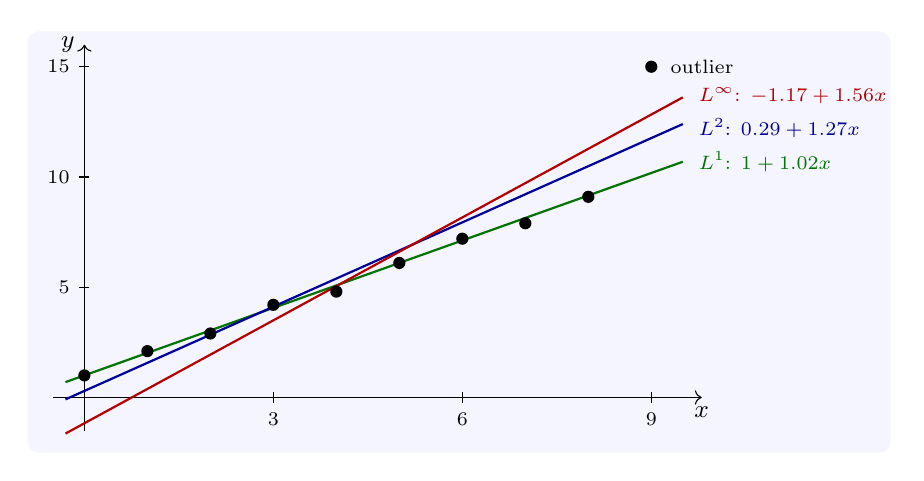
\begin{tikzpicture}[x=0.8cm,y=0.28cm]
\fill[blue!4,rounded corners=4pt] (-0.9,-2.5) rectangle (12.8,16.6);
\draw[->] (-0.5,0) -- (9.8,0) node[below,font=\small] {$x$};
\draw[->] (0,-1.5) -- (0,16) node[left,font=\small] {$y$};
\foreach \y in {5,10,15} \draw (0.08,\y) -- (-0.08,\y) node[left,font=\scriptsize] {$\y$};
\foreach \x in {3,6,9} \draw (\x,0.25) -- (\x,-0.25) node[below,font=\scriptsize] {$\x$};
\draw[green!45!black,thick] (-0.3,0.694) -- (9.5,10.69);
\draw[blue!60!black,thick] (-0.3,-0.088) -- (9.5,12.40);
\draw[red!70!black,thick] (-0.3,-1.639) -- (9.5,13.61);
\foreach \x/\y in {0/1.0,1/2.1,2/2.9,3/4.2,4/4.8,5/6.1,6/7.2,7/7.9,8/9.1,9/15.0} \fill (\x,\y) circle (2.2pt);
\node[font=\scriptsize,anchor=west] at (9.15,15.0) {outlier};
\node[font=\scriptsize,green!45!black,anchor=west] at (9.6,10.69) {$L^1$: $1 + 1.02x$};
\node[font=\scriptsize,blue!60!black,anchor=west] at (9.6,12.2) {$L^2$: $0.29 + 1.27x$};
\node[font=\scriptsize,red!70!black,anchor=west] at (9.6,13.7) {$L^\infty$: $-1.17 + 1.56x$};
\end{tikzpicture}
\caption{Three straight-line fits to ten points, the last an outlier. The least-absolute-deviations ($L^1$) fit, a linear programme, passes through the bulk of the data and ignores the outlier; least squares ($L^2$) is pulled towards it; the minimax ($L^\infty$) fit, also a linear programme, is pulled
furthest, since it balances the largest deviations (Software~\ref{sw:fits}).}
\label{fig:fits}
\end{figure}

\subsection{Linear programming in software}
\label{ssec:software1}

SciPy's \texttt{linprog} minimises $c^{\mathsf T}x$ subject to $A_{\text{ub}}x \leq b_{\text{ub}}$, $A_{\text{eq}}x = b_{\text{eq}}$ and bounds on each variable, using the HiGHS solvers. A maximisation is entered as the minimisation of $-c^{\mathsf T}x$, and a $\geq$ constraint by multiplying it by $-1$.

\begin{software}[Product mix and inspectors]
\label{sw:productmix}
Examples~\ref{ex:components} and \ref{ex:inspectors}:
{\small\begin{verbatim}
>>> import numpy as np
>>> from scipy.optimize import linprog
>>> c = [-20, -30]  # maximise 20 x1 + 30 x2: minimise -Z
>>> A = [[10, 40], [3, 2], [2, 3]]         # budget, machine, assembly
>>> b = [4000, 2000, 1400]
>>> r = linprog(c, A_ub=A, b_ub=b, method='highs')
>>> r.x, -r.fun, b - np.array(A) @ r.x     # plan, profit, unused resources
(array([400.,   0.]), 8000.0, array([  0., 800., 600.]))
>>> r = linprog([68.8, 68.0],  # inspectors: daily cost per inspector
...             A_ub=[[-320, -240]], b_ub=[-2000],   # at least 2000 pieces
...             bounds=[(0, 9), (0, 11)], method='highs')
>>> r.x, r.fun
(array([6.25, 0.  ]), 430.0)
\end{verbatim}}
\textbf{Reading the output.} The product mix makes $400$ of $C_1$ for a profit of $8000$; the slacks are $0$ for the budget and $800$ and $600$ hours of machine and assembly time. The inspection plan uses $6.25$ Grade~1 inspectors and no Grade~2, at Rs.~430 a day, a fractional answer that the model's divisibility
assumption allowed.

\textbf{MATLAB/Octave:} \texttt{linprog(-[20;30], [10 40; 3 2; 2 3], [4000; 2000; 1400], [], [], [0;0])}.
\end{software}

\begin{software}[A four-month plan]
\label{sw:multiperiod}
Example~\ref{ex:multiperiod}, with the twelve variables ordered as regular production, overtime and stock, and one balance equation per month:
{\small\begin{verbatim}
>>> d = np.array([100, 150, 200, 120])     # demand in four months
>>> T = len(d)  # variables: regular, overtime, stock
>>> cost = np.r_[10*np.ones(T), 14*np.ones(T), 2*np.ones(T)]
>>> Aeq = np.zeros((T, 3*T))
>>> for t in range(T):            # stock_{t-1} + R_t + O_t - stock_t = d_t
...     Aeq[t, t] = Aeq[t, T + t] = 1; Aeq[t, 2*T + t] = -1
...     if t > 0: Aeq[t, 2*T + t - 1] = 1
...
>>> bounds = [(0, 140)]*T + [(0, 40)]*T + [(0, None)]*T
>>> r = linprog(cost, A_eq=Aeq, b_eq=d, bounds=bounds, method='highs')
>>> r.x.reshape(3, T), r.fun               # rows: regular, overtime, stock
(array([[140., 140., 140., 120.],
       [  0.,   0.,  30.,   0.],
       [ 40.,  30.,   0.,   0.]]), 5960.0)
\end{verbatim}}
\textbf{Reading the output.} Regular production is $140$ in each of the first three months and $120$ in the last; overtime of $30$ is used only in month $3$; stocks of $40$ and $30$ are carried out of months $1$ and $2$ into the peak. The total cost is Rs.~5960. Checking month $3$: $30 + 140 + 30 - 0 = 200$.

\textbf{MATLAB/Octave:} the same matrices with \texttt{linprog(cost, [], [], Aeq, d, lb, ub)}.
\end{software}

\begin{software}[Fitting a line by linear programming]
\label{sw:fits}
The $L^\infty$ and $L^1$ fits of Figure~\ref{fig:fits} as linear programmes, with the free intercept and slope declared by the bounds \texttt{(None, None)}, and least squares for comparison:
{\small\begin{verbatim}
>>> xs = np.arange(10.0)
>>> ys = np.array([1.0, 2.1, 2.9, 4.2, 4.8, 6.1, 7.2, 7.9, 9.1, 15.0])
>>> n = len(xs)                   # L-infinity fit: min t, |y - a - bx| <= t
>>> one = np.ones(n)
>>> A = np.r_[np.c_[-one, -xs, -one], np.c_[one, xs, -one]]
>>> r = linprog([0, 0, 1], A_ub=A, b_ub=np.r_[-ys, ys],
...             bounds=[(None, None)]*2 + [(0, None)], method='highs')
>>> cheb = r.x[:2]
>>> I = np.eye(n)  # L1 fit: min sum e_i, |y_i - a - b x_i| <= e_i
>>> A = np.r_[np.c_[-np.ones(n), -xs, -I], np.c_[np.ones(n), xs, -I]]
>>> r = linprog(np.r_[0, 0, np.ones(n)], A_ub=A, b_ub=np.r_[-ys, ys],
...             bounds=[(None, None)]*2 + [(0, None)]*n, method='highs')
>>> l1 = r.x[:2]
>>> ls = np.polyfit(xs, ys, 1)[::-1]       # least squares, for comparison
>>> np.round(np.array([l1, ls, cheb]), 4)  # rows: L1, L2, L-infinity; (a, b)
array([[ 1.    ,  1.02  ],
       [ 0.2945,  1.2745],
       [-1.1722,  1.5556]])
\end{verbatim}}
\textbf{Reading the output.} The $L^1$ line is $1 + 1.02x$, close to the trend of the first nine points; least squares gives $0.29 + 1.27x$ and the Chebyshev fit $-1.17 + 1.56x$. One bad point moves the slope by $25\%$ and $53\%$ for the last two. The $L^1$ fit is the regression analogue of the median, and like it, robust.

\textbf{MATLAB/Octave:} \texttt{linprog} with the same stacked constraint matrices.
\end{software}

\subsection{Practice Problems}

\begin{problem}
\label{prob:inspectorsint}
In Example~\ref{ex:inspectors}, find the cheapest assignment in which both numbers of inspectors are whole, by checking the possible numbers of Grade~1 inspectors, and compare it with the LP value Rs.~430 and with rounding $6.25$ up to $7$.
\end{problem}

\begin{solution}
For each $x_1 = 0, \ldots, 7$ take the least $x_2$ with $320x_1 + 240x_2 \geq 2000$. The costs are: $x_1 = 7, x_2 = 0$: $481.6$; $6, 1$: $480.8$; $5, 2$: $480.0$; $4, 3$: $479.2$; $3, 5$: $546.4$; $2, 6$: $545.6$; $1, 7$: $544.8$; $0, 9$: $612$. The best is $4$ Grade~1 and $3$ Grade~2 inspectors at
Rs.~479.2, which inspect exactly $2000$ pieces. Rounding the LP solution up gives Rs.~481.6; the integer optimum mixes the grades, which the LP never does. The gap between Rs.~430 and Rs.~479.2 is the cost of indivisibility.
\end{solution}

\begin{problem}
Complete Example~\ref{ex:feedmix}: write the model, solve it graphically or by any method, and state how much wheat and barley are used.
\end{problem}

\begin{solution}
Maximise $0.383x_1 + 0.367x_2$ subject to $2x_1 + x_2 \leq 3000$, $x_1 + 2x_2 \leq 3600$, $x \geq 0$. The two constraints meet where $x_1 = 800$, $x_2 = 1400$, with profit $0.383 \times 800 + 0.367 \times 1400 = 820$. The other vertices give $0.383 \times 1500 = 575$ at $(1500, 0)$ and $0.367 \times 1800 = 660$ at
$(0, 1800)$, so the optimum is $800$\,kg of Fertilex and $1400$\,kg of Multiplex, using all $1000$\,kg of wheat and all $1200$\,kg of barley.
\end{solution}

\begin{problem}
A firm makes two products over three months. Product~1 sells for Rs.~14 and costs Rs.~10 to make; product~2 sells for Rs.~11 and costs Rs.~8. Each unit of product~1 needs $0.5$, $0.3$ and $0.2$ hours in departments $A$, $B$, $C$, and each unit of product~2 needs $0.3$, $0.4$ and $0.1$ hours, with $500$, $400$ and
$200$ hours available. The firm has Rs.~3 lakh of its own funds and may borrow up to Rs.~2 lakh at $20\%$ a year for the three months. Formulate a model to maximise profit after interest, with $x_3$ the amount borrowed, assuming production costs must be paid from funds available.
\end{problem}

\begin{solution}
Interest for three months is $0.20 \times \frac3{12} = 0.05$ per rupee. Maximise $Z = 4x_1 + 3x_2 - 0.05x_3$ subject to $0.5x_1 + 0.3x_2 \leq 500$, $0.3x_1 + 0.4x_2 \leq 400$, $0.2x_1 + 0.1x_2 \leq 200$ (capacity); $10x_1 + 8x_2 \leq 300\,000 + x_3$ (funds); $0 \leq x_3 \leq 200\,000$. Here the
capacity constraints bind long before the funds do (at most $1000$ units of product~1 cost only Rs.~10\,000), so $x_3 = 0$ at the optimum: borrowing is worth while only when money, not capacity, is scarce. The optimum is $x_1 = 727.3$, $x_2 = 454.5$, where departments $A$ and $C$ are fully used, with profit Rs.~4272.7.
\end{solution}

\begin{problem}
Write the problem ``minimise $|x_1 - 2| + |x_2 + 1|$ subject to $x_1 + x_2 \geq 3$, $x_1, x_2$ free'' as a linear programme in standard form.
\end{problem}

\begin{solution}
Introduce $e_1, e_2 \geq 0$: minimise $e_1 + e_2$ subject to $-e_1 \leq x_1 - 2 \leq e_1$, $-e_2 \leq x_2 + 1 \leq e_2$, $x_1 + x_2 \geq 3$. For standard form, write $x_j = x_j^+ - x_j^-$ and add a slack or surplus variable to each of the five inequalities, giving $5$ equations in $4 + 2 + 5 = 11$ non-negative
variables. The optimal value is $2$, attained for example at $x = (2, 1)$.
\end{solution}

\begin{problem}
A hospital needs at least $17$, $13$, $15$, $19$, $14$, $16$ and $11$ nurses on the seven days of the week, Monday to Sunday. Each nurse works five consecutive days and then has two days off. Formulate the problem of minimising the number of nurses employed.
\end{problem}

\begin{solution}
Let $x_j$ be the number of nurses whose five-day spell starts on day $j$ ($j = 1$ for Monday). A nurse works on day $i$ if the spell started on day $i$ or one of the four days before, cyclically. Minimise $\sum_{j = 1}^7x_j$ subject to, for Monday, $x_1 + x_4 + x_5 + x_6 + x_7 \geq 17$, for Tuesday
$x_1 + x_2 + x_5 + x_6 + x_7 \geq 13$, and so on cyclically, with $x_j \geq 0$ and integer. Summing the seven constraints, each $x_j$ appears five times, so $5\sum x_j \geq 105$ and at least $21$ nurses are needed.
\end{solution}

\begin{problem}
Explain which of the four assumptions of linear programming fails in each case, and how the model might be repaired: (a) a machine must be set up at a fixed cost before any units are made; (b) the price of a product falls as more is sold; (c) the yield of a crop depends on next season's rainfall.
\end{problem}

\begin{solution}
(a) Proportionality: the cost is $F + cx$ for $x > 0$ and $0$ for $x = 0$. Repair with a binary variable $y$, cost $Fy + cx$ and $x \leq My$ (see the section on integer programming). (b) Proportionality: revenue $p(x)x$ is non-linear; if it is concave it can be approximated piecewise linearly for maximisation, otherwise use
non-linear programming. (c) Certainty: the coefficient is random; use expected values with sensitivity analysis, or a stochastic model with scenarios.
\end{solution}

%======================================================================
\section{The Geometry of Linear Programming}
\label{sec:geometry}

The feasible region of a linear programme is an intersection of half-spaces, a convex polyhedron, and a linear objective is maximised over it at a corner. This one geometric fact is the reason linear programming can be solved exactly: it reduces a search over infinitely many points to a search over finitely many
vertices, and the simplex method of the next section is a systematic way of walking from vertex to vertex. This section makes the fact precise, with the algebraic description of vertices as basic feasible solutions, and uses it to solve small problems graphically.

\subsection{Convex sets and polyhedra}
\label{ssec:convex}

\begin{defn}
A set $S \subseteq \mathbb R^n$ is \textbf{convex} if it contains the segment between any two of its points: $x, y \in S$ and $0 \leq \lambda \leq 1$ imply $\lambda x + (1 - \lambda)y \in S$. A \textbf{convex combination} of $x^1, \ldots, x^k$ is $\sum\lambda_ix^i$ with $\lambda_i \geq 0$ and $\sum\lambda_i = 1$. A
\textbf{polyhedron} is a set $\{x : Gx \leq h\}$, the intersection of finitely many closed half-spaces.
\end{defn}

A half-space $\{x : g^{\mathsf T}x \leq \eta\}$ is convex, since $g^{\mathsf T}(\lambda x + (1 - \lambda)y) = \lambda g^{\mathsf T}x + (1 - \lambda)g^{\mathsf T}y \leq \eta$, and an intersection of convex sets is convex. So every polyhedron, in particular the feasible region of every LP, is convex. The standard-form region
$P = \{x : Ax = b, x \geq 0\}$ is a polyhedron, since an equation is two inequalities.

\begin{defn}
A point $x$ of a convex set $S$ is an \textbf{extreme point} if it is not a convex combination of two other points of $S$: $x = \lambda y + (1 - \lambda)z$ with $y, z \in S$ and $0 < \lambda < 1$ implies $y = z = x$. For a polyhedron, the extreme points are its \textbf{vertices}.
\end{defn}

\subsection{Basic feasible solutions}
\label{ssec:bfs}

For computation we need an algebraic description of the vertices of $P = \{x : Ax = b, x \geq 0\}$, where $A$ is $m \times n$ of rank $m$.

\begin{defn}
Choose $m$ linearly independent columns of $A$, forming the \textbf{basis matrix} $B$; the corresponding variables are \textbf{basic}, the others \textbf{non-basic}. Setting the non-basic variables to $0$ and solving $Bx_B = b$ gives a \textbf{basic solution}. If also $x_B = B^{-1}b \geq 0$, it is a
\textbf{basic feasible solution} (BFS). It is \textbf{degenerate} if some basic variable is $0$.
\end{defn}

\begin{thm}
\label{thm:bfs}
A point $x \in P$ is an extreme point of $P$ if and only if the columns $A_j$ with $x_j > 0$ are linearly independent; and this holds if and only if $x$ is a basic feasible solution.
\end{thm}

\begin{proof}
Let $J = \{j : x_j > 0\}$. Suppose the columns $A_j$, $j \in J$, are dependent: $\sum_{j \in J}d_jA_j = 0$ with $d \neq 0$, $d_j = 0$ for $j \notin J$. Then $Ad = 0$, and for small $\varepsilon > 0$ both $x \pm \varepsilon d$ are in $P$, since their components outside $J$ are $0$ and those in $J$ stay positive. As
$x = \frac12(x + \varepsilon d) + \frac12(x - \varepsilon d)$, $x$ is not extreme.

Conversely, suppose the columns in $J$ are independent and $x = \lambda y + (1 - \lambda)z$ with $y, z \in P$, $0 < \lambda < 1$. For $j \notin J$, $0 = \lambda y_j + (1 - \lambda)z_j$ with $y_j, z_j \geq 0$ forces $y_j = z_j = 0$. Then $A(y - x) = 0$ with $y - x$ supported in $J$, and independence gives $y = x$, and
likewise $z = x$. So $x$ is extreme.

Finally, independent columns in $J$ can be extended to a basis of $m$ columns (since $A$ has rank $m$), and $x$ is the basic solution for that basis, feasible since $x \geq 0$; and a BFS has its positive components among independent basic columns.
\end{proof}

At a degenerate BFS, $J$ has fewer than $m$ columns and can be extended to a basis in several ways, so one vertex corresponds to several bases. This harmless-looking fact is the source of the difficulties with cycling in the simplex method.

\begin{thm}[Fundamental theorem of linear programming]
\label{thm:fundamental}
Consider the LP: minimise $c^{\mathsf T}x$ over $P = \{x : Ax = b, x \geq 0\}$.
\begin{enumerate}[label=(\roman*)]
\item If $P$ is non-empty, it has a basic feasible solution.
\item If the LP has an optimal solution, it has an optimal basic feasible solution.
\end{enumerate}
\end{thm}

\begin{proof}
(ii) Among the optimal solutions choose one, $x$, with the fewest positive components, and let $J$ be its support. If the columns in $J$ were dependent, take $d \neq 0$ supported in $J$ with $Ad = 0$. Then $x + \varepsilon d$ is feasible for all small $|\varepsilon|$, so by optimality $c^{\mathsf T}d = 0$,
since otherwise one sign of $\varepsilon$ would decrease the objective. Replacing $d$ by $-d$ if necessary, some $d_j < 0$; increase $\varepsilon$ from $0$ until the first component $x_j + \varepsilon d_j$ reaches $0$. The new point is feasible and optimal, since $c^{\mathsf T}d = 0$, with fewer positive components,
a contradiction. So the columns in $J$ are independent, and $x$ is a BFS by Theorem~\ref{thm:bfs}. (i) is the same argument with any feasible point of minimal support, without the objective.
\end{proof}

There are at most $\binom nm$ bases, so an LP could in principle be solved by computing every basic solution and comparing (Software~\ref{sw:bases}). For $n = 50$ and $m = 25$ that is $\binom{50}{25} = 1.26 \times 10^{14}$ systems: enumeration is hopeless, and the simplex method visits only a few of them. The full structure is given by
the \textbf{representation theorem} of Minkowski and Weyl: a polyhedron with at least one vertex is the set of points $\sum\lambda_iv^i + \sum\mu_jw^j$, with $\lambda_i \geq 0$, $\sum\lambda_i = 1$, $\mu_j \geq 0$, where $v^i$ are its vertices and $w^j$ the directions of its unbounded edges (extreme rays). A bounded polyhedron is the convex hull of
its vertices.

\subsection{The graphical method}
\label{ssec:graphical}

With two variables the feasible region can be drawn. Plot each constraint as a line, shade the side that satisfies it, and identify the polygon common to all. Draw the \textbf{iso-profit lines} $c^{\mathsf T}x = Z$; they are parallel, and $Z$ increases in the direction of the gradient $c$. Slide the line in that
direction as far as it still meets the region; the last point of contact is optimal, and by Theorem~\ref{thm:fundamental} it may be taken to be a vertex, so it suffices to evaluate $Z$ at the vertices.

\begin{exa}
\label{ex:graphical}
Maximise $Z = 10x_1 + 15x_2$ subject to $2x_1 + x_2 \leq 26$, $2x_1 + 4x_2 \leq 56$, $-x_1 + x_2 \leq 5$, $x_1, x_2 \geq 0$. The region is the pentagon with vertices $O(0, 0)$, $A(13, 0)$, $B(8, 10)$, $C(6, 11)$, $D(0, 5)$ (Figure~\ref{fig:graphical}), where $Z = 0$, $130$, $230$, $225$ and $75$. The maximum is
$Z = 230$ at $B$, where the first two constraints are tight and the third has slack $3$.
\end{exa}

\begin{figure}[H]
\centering
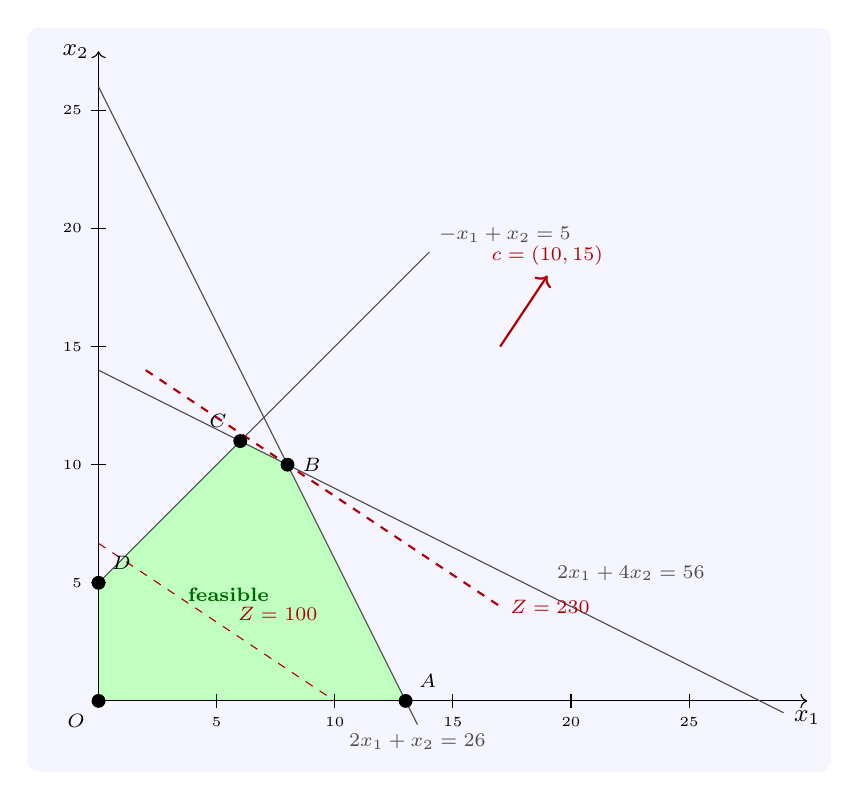
\begin{tikzpicture}[x=0.3cm,y=0.3cm]
\fill[blue!4,rounded corners=4pt] (-3,-3) rectangle (31,28.5);
\fill[green!25] (0,0) -- (13,0) -- (8,10) -- (6,11) -- (0,5) -- cycle;
\draw[->] (0,0) -- (30,0) node[below,font=\small] {$x_1$};
\draw[->] (0,0) -- (0,27.5) node[left,font=\small] {$x_2$};
\foreach \v in {5,10,15,20,25} {\draw (\v,0.3) -- (\v,-0.3) node[below,font=\tiny] {$\v$}; \draw (0.3,\v) -- (-0.3,\v) node[left,font=\tiny] {$\v$};}
\draw[black!70] (0,26) -- (13.5,-1) node[below,font=\scriptsize] {$2x_1 + x_2 = 26$};
\draw[black!70] (0,14) -- (29,-0.5);
\node[font=\scriptsize,black!70,anchor=west] at (19,5.4) {$2x_1 + 4x_2 = 56$};
\draw[black!70] (0,5) -- (14,19) node[above right,font=\scriptsize] {$-x_1 + x_2 = 5$};
\draw[red!70!black,dashed] (0,6.667) -- (10,0) node[pos=0.55,above right,font=\scriptsize] {$Z = 100$};
\draw[red!70!black,thick,dashed] (2,14) -- (17,4) node[right,font=\scriptsize] {$Z = 230$};
\draw[->,red!70!black,thick] (17,15) -- (19,18) node[above,font=\scriptsize] {$c = (10, 15)$};
\foreach \p/\q/\l/\a in {0/0/O/below left, 13/0/A/above right, 8/10/B/right, 6/11/C/above left, 0/5/D/above right}
  \fill (\p,\q) circle (2.5pt) node[\a=2pt,font=\scriptsize] {$\l$};
\node[font=\scriptsize\bfseries,green!40!black] at (5.5,4.5) {feasible};
\end{tikzpicture}
\caption{The graphical method for Example~\ref{ex:graphical}. The feasible region is the shaded pentagon. The iso-profit lines $10x_1 + 15x_2 = Z$ move in the direction $c$ as $Z$ increases; the last contact with the region is the vertex $B(8, 10)$, where $Z = 230$.}
\label{fig:graphical}
\end{figure}

The method also shows the four things that can happen in an LP.
\begin{itemize}
\item \textbf{A unique optimum} at a vertex, as above.
\item \textbf{Multiple optima}, when the objective is parallel to an edge of the region at which it is optimal. With $Z = x_1 + 2x_2$ in Example~\ref{ex:graphical}, parallel to $2x_1 + 4x_2 = 56$, every point of the edge $BC$ gives $Z = 28$. The optimal set is always convex: it is a face of the polyhedron.
\item \textbf{Unboundedness}, when the region is unbounded in a direction along which the objective improves without limit.
\item \textbf{Infeasibility}, when the constraints are inconsistent, as with $x_1 + x_2 \leq 2$ and $x_1 + x_2 \geq 3$.
\end{itemize}
A constraint that can be deleted without changing the region is \textbf{redundant}. When three or more constraint lines pass through one vertex in the plane, the vertex is degenerate in the sense of the last subsection.

\subsection{Geometry in software}
\label{ssec:software2}

\begin{software}[Enumerating vertices]
\label{sw:vertices}
For Example~\ref{ex:graphical}, the intersection of every pair of the five constraint lines (the last two being $x_1 = 0$ and $x_2 = 0$), whether it is feasible, and the objective at the feasible ones; then the LP solution for comparison:
{\small\begin{verbatim}
>>> import numpy as np
>>> from itertools import combinations
>>> from scipy.optimize import linprog
>>> G = np.array([[2, 1], [2, 4], [-1, 1], [-1, 0], [0, -1]])   # G x <= h,
>>> h = np.array([26, 56, 5, 0, 0])        # the last two rows are x1, x2 >= 0
>>> c = np.array([10, 15])
>>> for i, j in combinations(range(5), 2): # every pair of constraint lines
...     M = G[[i, j]]
...     if abs(np.linalg.det(M)) < 1e-12: continue        # parallel lines
...     v = np.linalg.solve(M, h[[i, j]]) + 0.0
...     ok = np.all(G @ v <= h + 1e-9)
...     print((i + 1, j + 1), np.round(v, 3), 'vertex' if ok else '-',
...           round(c @ v, 2) if ok else '')
...
(1, 2) [ 8. 10.] vertex 230.0
(1, 3) [ 7. 12.] - 
(1, 4) [ 0. 26.] - 
(1, 5) [13.  0.] vertex 130.0
(2, 3) [ 6. 11.] vertex 225.0
(2, 4) [ 0. 14.] - 
(2, 5) [28.  0.] - 
(3, 4) [0. 5.] vertex 75.0
(3, 5) [-5.  0.] - 
(4, 5) [0. 0.] vertex 0.0
>>> r = linprog(-c, A_ub=G[:3], b_ub=h[:3], method='highs'); r.x, -r.fun
(array([ 8., 10.]), 230.0)
\end{verbatim}}
\textbf{Reading the output.} Of the ten intersections, five satisfy all the constraints; they are the vertices $B$, $A$, $C$, $D$, $O$ of Figure~\ref{fig:graphical}. The other five lie outside the region: $(7, 12)$ violates the second constraint, $(28, 0)$ the first. The largest objective value, $230$ at $(8, 10)$, is
what \texttt{linprog} returns.

\textbf{MATLAB/Octave:} \texttt{nchoosek(1:5, 2)} lists the pairs.
\end{software}

\begin{software}[What can go wrong]
\label{sw:cases}
\texttt{linprog} on an unbounded problem (with $x_1$ free), an infeasible one, and Example~\ref{ex:graphical} with the objective $x_1 + 2x_2$, which has a tie:
{\small\begin{verbatim}
>>> cases = {     # linprog status: 0 optimal, 2 infeasible, 3 unbounded
...   'unbounded':  dict(c=[-1, 4], A_ub=[[-3, 1], [1, 2], [0, 1]],
...                      b_ub=[6, 4, -3], bounds=[(None, None)]*2),
...   'infeasible': dict(c=[1, 1], A_ub=[[1, 1], [-1, -1]], b_ub=[2, -3]),
...   'tied':       dict(c=[-1, -2], A_ub=G[:3], b_ub=h[:3])}
>>> for name, kw in cases.items():
...     r = linprog(method='highs', **kw)
...     print(f"{name:10s} status {r.status}", r.x if r.status == 0 else '',
...           -r.fun if r.status == 0 else '')
...
unbounded  status 3  
infeasible status 2  
tied       status 0 [ 6. 11.] 28.0
\end{verbatim}}
\textbf{Reading the output.} The solver reports status $3$ (unbounded) and $2$ (infeasible) instead of a solution. For the tied objective it returns one optimal vertex, $C(6, 11)$, with $Z = 28$; the vertex $B(8, 10)$ and every point between are equally good, and a solver gives no warning of this, which
sensitivity analysis will detect.

\textbf{MATLAB/Octave:} the \texttt{exitflag} output, $-2$ for infeasible and $-3$ for unbounded.
\end{software}

\begin{software}[Bases and vertices]
\label{sw:bases}
Minimise $20x_1 + 10x_2$ subject to $x_1 + 2x_2 \leq 40$, $3x_1 + x_2 \geq 30$, $4x_1 + 3x_2 \geq 60$, $x \geq 0$, in standard form with one slack and two surplus variables: all $\binom53 = 10$ choices of three basic columns, keeping the feasible ones:
{\small\begin{verbatim}
>>> A = np.array([[1, 2, 1, 0, 0],         # min 20 x1 + 10 x2, standard form:
...               [3, 1, 0, -1, 0],        # x1 + 2 x2 + s1 = 40
...               [4, 3, 0, 0, -1]])       # 3 x1 + x2 - s2 = 30, and so on
>>> b = np.array([40, 30, 60]); cost = np.array([20, 10, 0, 0, 0])
>>> count = feasible = 0
>>> for B in combinations(range(5), 3):  # every choice of three basic columns
...     AB = A[:, B]
...     if abs(np.linalg.det(AB)) < 1e-12: continue
...     count += 1; xB = np.linalg.solve(AB, b)
...     if np.all(xB >= -1e-9):
...         feasible += 1; x = np.zeros(5); x[list(B)] = xB
...         print(B, np.round(x[:2], 3), round(cost @ x, 2))
...
(0, 1, 2) [ 6. 12.] 240.0
(0, 1, 4) [ 4. 18.] 260.0
(0, 2, 3) [15.  0.] 300.0
(0, 3, 4) [40.  0.] 800.0
>>> count, feasible
(10, 4)
\end{verbatim}}
\textbf{Reading the output.} All ten column triples are bases, and four give basic \emph{feasible} solutions: the vertices $(6, 12)$, $(4, 18)$, $(15, 0)$ and $(40, 0)$, with costs $240$, $260$, $300$ and $800$. The minimum is $240$ at $(6, 12)$, where the two $\geq$ constraints are tight.

\textbf{MATLAB/Octave:} \texttt{nchoosek(1:5, 3)} and \texttt{A(:, B) \textbackslash\ b}.
\end{software}

\subsection{Practice Problems}

\begin{problem}
Solve graphically: maximise $Z = 7x_1 + 3x_2$ subject to $x_1 + 2x_2 \geq 3$, $x_1 + x_2 \leq 4$, $x_1 \leq \frac52$, $x_2 \leq \frac32$, $x \geq 0$. Show that the optimal vertex is degenerate.
\end{problem}

\begin{solution}
The vertices are $A(\frac52, \frac14)$, $B(\frac52, \frac32)$ and $C(0, \frac32)$, with $Z = \frac{73}4$, $22$ and $\frac92$. The maximum is $22$ at $B$. Three constraint lines pass through $B$: $x_1 = \frac52$, $x_2 = \frac32$ and $x_1 + x_2 = 4$. In standard form, with four slack or surplus variables and $m = 4$, the BFS at
$B$ has $x_1, x_2$ and the surplus of the first constraint positive and the slacks of the other three zero, so one basic variable is zero: degenerate, and $B$ is given by three different bases.
\end{solution}

\begin{problem}
Show that the problem: minimise $-x_1 + 4x_2$ subject to $-3x_1 + x_2 \leq 6$, $x_1 + 2x_2 \leq 4$, $x_2 \leq -3$, with $x_1$ free in sign, is unbounded.
\end{problem}

\begin{solution}
Take $x_2 = -t$ with $t \geq 3$ and $x_1 = 4 + 2t$. Then $-3x_1 + x_2 = -12 - 7t \leq 6$ and $x_1 + 2x_2 = 4$, so the point is feasible, and the objective is $-4 - 2t - 4t = -4 - 6t \to -\infty$. The region contains the ray $(4, 0) + t(2, -1)$, $t \geq 3$, along which the objective
decreases; Software~\ref{sw:cases} reports status $3$.
\end{solution}

\begin{problem}
Prove that the set of optimal solutions of an LP is convex.
\end{problem}

\begin{solution}
If $x$ and $y$ are optimal with value $z^*$, then $\lambda x + (1 - \lambda)y$ is feasible, since the feasible region is convex, and its objective value is $\lambda z^* + (1 - \lambda)z^* = z^*$ by linearity, so it is optimal.
\end{solution}

\begin{problem}
Find all basic solutions of $x_1 + x_2 + x_3 = 4$, $x_1 - x_2 + 2x_4 = 2$, decide which are feasible, and identify any degenerate ones.
\end{problem}

\begin{solution}
There are $\binom42 = 6$ choices of basis. $\{x_1, x_2\}$: $x = (3, 1, 0, 0)$, feasible. $\{x_1, x_3\}$: $x_1 = 2$, $x_3 = 2$, feasible. $\{x_1, x_4\}$: $x_1 = 4$, $x_4 = -1$, infeasible. $\{x_2, x_3\}$: $x_2 = -2$, infeasible. $\{x_2, x_4\}$: $x_2 = 4$, $x_4 = 3$, feasible. $\{x_3, x_4\}$: $x_3 = 4$, $x_4 = 1$,
feasible. None is degenerate, since every basic variable in the feasible ones is positive.
\end{solution}

\begin{problem}
In Example~\ref{ex:graphical}, for which values of $c_2$ does the vertex $B(8, 10)$ remain optimal for the objective $10x_1 + c_2x_2$?
\end{problem}

\begin{solution}
$B$ is optimal while the slope of the iso-profit lines, $-10/c_2$, lies between the slopes of the two constraints tight at $B$: $-2$ for $2x_1 + x_2 = 26$ and $-\frac12$ for $2x_1 + 4x_2 = 56$. So $-2 \leq -10/c_2 \leq -\frac12$, that is $5 \leq c_2 \leq 20$. At $c_2 = 20$ the edge $BC$ is also optimal, and above it $C$ takes over;
at $c_2 = 5$ the edge $AB$ is optimal.
\end{solution}

\begin{problem}
Show that the polyhedron $\{x \in \mathbb R^2 : x_1 + x_2 \geq 1,\ x \geq 0\}$ has two vertices and two extreme rays, and write the point $(3, 2)$ in the form given by the representation theorem.
\end{problem}

\begin{solution}
The vertices are $(1, 0)$ and $(0, 1)$, and the unbounded edges point in the directions $(1, 0)$ and $(0, 1)$. Then $(3, 2) = 1\cdot(1, 0) + 2\cdot(1, 0) + 2\cdot(0, 1)$, a convex combination of vertices (here just one, with $\lambda = 1$) plus $\mu_1 = 2$, $\mu_2 = 2$ times the rays. The representation is not
unique: $\frac12(1, 0) + \frac12(0, 1) + \frac52(1, 0) + \frac32(0, 1)$ also works.
\end{solution}

%======================================================================
\section{The Simplex Method}
\label{sec:simplex}

By the fundamental theorem, an optimal solution of an LP can be found among its basic feasible solutions. Dantzig's \textbf{simplex method} (1947) moves from one BFS to an adjacent one with a better objective value, until no neighbour is better. Each move is a \textbf{pivot}: one variable enters the basis and
one leaves. This section derives the method from the algebra of bases, proves that it stops at an optimum, shows how to start it, and explains the two things that can go wrong, degeneracy and exponential running time.

\subsection{Reduced costs and the optimality test}
\label{ssec:reducedcosts}

Consider the standard-form problem: minimise $c^{\mathsf T}x$ subject to $Ax = b$, $x \geq 0$, and a BFS with basis matrix $B$, so that $x_B = B^{-1}b \geq 0$ and $x_N = 0$. Every solution of $Ax = b$ satisfies $Bx_B + Nx_N = b$, so
\[
x_B = B^{-1}b - B^{-1}Nx_N, \qquad c^{\mathsf T}x = c_B^{\mathsf T}B^{-1}b + \sum_{j \in N}\bar c_jx_j, \qquad \bar c_j = c_j - c_B^{\mathsf T}B^{-1}A_j .
\]
The number $\bar c_j$ is the \textbf{reduced cost} of the non-basic variable $x_j$: the rate at which the objective changes when $x_j$ is increased from $0$ and the basic variables adjust to keep $Ax = b$. (Sharma, following a common textbook convention for maximisation, writes $c_j - z_j$ with
$z_j = c_B^{\mathsf T}B^{-1}A_j$; it is the same quantity.)

\begin{thm}[Optimality test]
\label{thm:optimality}
If $\bar c_j \geq 0$ for every non-basic $j$, the BFS is optimal.
\end{thm}

\begin{proof}
For any feasible $y$, $y_N \geq 0$, so by the identity above $c^{\mathsf T}y = c_B^{\mathsf T}B^{-1}b + \sum_{j \in N}\bar c_jy_j \geq c_B^{\mathsf T}B^{-1}b = c^{\mathsf T}x$.
\end{proof}

If some $\bar c_j < 0$, increasing $x_j$ improves the objective. Put $u = B^{-1}A_j$; increasing $x_j$ to $\theta$ changes the basic variables to $x_B - \theta u$. They stay non-negative as long as $\theta \leq x_{B(i)}/u_i$ for every $i$ with $u_i > 0$, which gives the \textbf{ratio test}
\[
\theta^* = \min\Bigl\{\frac{x_{B(i)}}{u_i} : u_i > 0\Bigr\} .
\]

\begin{thm}[A pivot]
\label{thm:pivot}
Let $\bar c_j < 0$.
\begin{enumerate}[label=(\roman*)]
\item If $u = B^{-1}A_j \leq 0$, the LP is unbounded: $x + \theta d$ is feasible for all $\theta \geq 0$, where $d_j = 1$, $d_B = -u$ and $d$ is $0$ elsewhere, and its cost $c^{\mathsf T}x + \theta\bar c_j \to -\infty$.
\item Otherwise, let the minimum in the ratio test be attained at row $\ell$. Replacing the basic variable $x_{B(\ell)}$ by $x_j$ gives a new basis, the new BFS is $x + \theta^*d$, and its cost is $c^{\mathsf T}x + \theta^*\bar c_j \leq c^{\mathsf T}x$, with strict inequality if $\theta^* > 0$.
\end{enumerate}
\end{thm}

\begin{proof}
$Ad = A_j - Bu = 0$, so $A(x + \theta d) = b$, and $x + \theta d \geq 0$ for $0 \leq \theta \leq \theta^*$ by the ratio test (for all $\theta \geq 0$ in case (i)); its cost is $c^{\mathsf T}x + \theta(c_j - c_B^{\mathsf T}u) = c^{\mathsf T}x + \theta\bar c_j$. In case (ii), at $\theta = \theta^*$ the variable $x_{B(\ell)}$ becomes $0$. The new
columns are independent: $A_j = Bu$ with $u_\ell > 0$, so $A_j$ is not in the span of the other basic columns. So the new point is a BFS.
\end{proof}

\begin{thm}[Finite termination]
\label{thm:termination}
If every BFS is non-degenerate, the simplex method stops after finitely many pivots, either with an optimal BFS or with a proof of unboundedness.
\end{thm}

\begin{proof}
Without degeneracy every $\theta^* > 0$, so each pivot strictly decreases the cost. Hence no basis is visited twice, and there are at most $\binom nm$ bases.
\end{proof}

\subsection{The tableau}
\label{ssec:tableau}

By hand, the computation is organised in a \textbf{tableau}: the rows of $[B^{-1}A \mid B^{-1}b]$, one per basic variable, and an objective row holding the reduced costs and the current value. A pivot on row $\ell$ and column $j$ divides row $\ell$ by the pivot element and subtracts multiples of it from the other rows,
including the objective row, so that column $j$ becomes a unit vector. For a maximisation written with slack variables, the objective row starts as $-c$, and the tableau is optimal when the objective row has no negative entries.

\begin{exa}
\label{ex:tableau}
For Example~\ref{ex:graphical}, add slacks $s_1, s_2, s_3$. The initial tableau, with basis $\{s_1, s_2, s_3\}$ at the origin, and the final one are
\begin{center}
\small
\begin{tabular}{c|rrrrr|r}
basic & $x_1$ & $x_2$ & $s_1$ & $s_2$ & $s_3$ & rhs \\
\hline
$s_1$ & $2$ & $1$ & $1$ & $0$ & $0$ & $26$ \\
$s_2$ & $2$ & $4$ & $0$ & $1$ & $0$ & $56$ \\
$s_3$ & $-1$ & $1$ & $0$ & $0$ & $1$ & $5$ \\
\hline
$Z$ & $-10$ & $-15$ & $0$ & $0$ & $0$ & $0$
\end{tabular}
\qquad
\begin{tabular}{c|rrrrr|r}
basic & $x_1$ & $x_2$ & $s_1$ & $s_2$ & $s_3$ & rhs \\
\hline
$s_3$ & $0$ & $0$ & $1$ & $-\frac12$ & $1$ & $3$ \\
$x_1$ & $1$ & $0$ & $\frac23$ & $-\frac16$ & $0$ & $8$ \\
$x_2$ & $0$ & $1$ & $-\frac13$ & $\frac13$ & $0$ & $10$ \\
\hline
$Z$ & $0$ & $0$ & $\frac53$ & $\frac{10}3$ & $0$ & $230$
\end{tabular}
\end{center}
With Dantzig's rule (enter the most negative entry of the objective row), $x_2$ enters first; the ratios are $26$, $14$ and $5$, so $s_3$ leaves and the method moves to $D(0, 5)$. Then $x_1$ enters and $s_1$ leaves, at $C(6, 11)$, and finally $s_3$ re-enters and $s_2$ leaves, at $B(8, 10)$ (Figure~\ref{fig:path},
Software~\ref{sw:tableau}). In the final tableau the objective row is non-negative, so $B$ is optimal. Its entries $\frac53$ and $\frac{10}3$ under $s_1$ and $s_2$ are the amounts by which $Z$ would rise per extra unit of the first and second resource: the \textbf{shadow prices}, which the section on duality interprets.
\end{exa}

\begin{figure}[H]
\centering
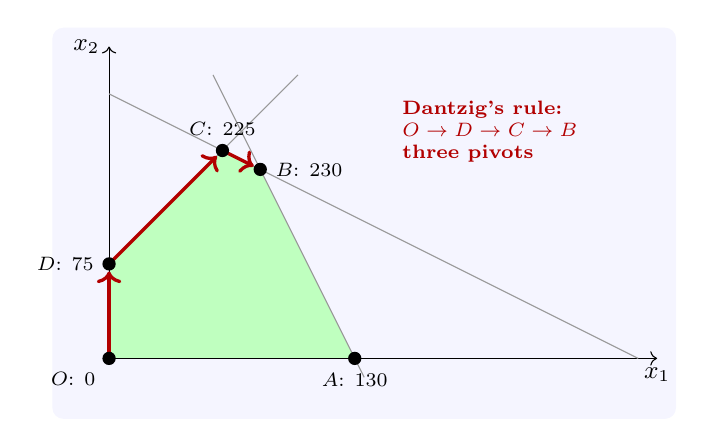
\begin{tikzpicture}[x=0.24cm,y=0.24cm]
\fill[blue!4,rounded corners=4pt] (-3,-3.2) rectangle (30,17.5);
\fill[green!25] (0,0) -- (13,0) -- (8,10) -- (6,11) -- (0,5) -- cycle;
\draw[->] (0,0) -- (29,0) node[below,font=\small] {$x_1$};
\draw[->] (0,0) -- (0,16.5) node[left,font=\small] {$x_2$};
\draw[black!40] (0,14) -- (28,0); \draw[black!40] (5.5,15) -- (13.5,-1); \draw[black!40] (0,5) -- (10,15);
\draw[->,red!70!black,very thick] (0,0) -- (0,4.6);
\draw[->,red!70!black,very thick] (0,5) -- (5.7,10.7);
\draw[->,red!70!black,very thick] (6,11) -- (7.65,10.17);
\foreach \p/\q/\l/\z/\a in {0/0/O/0/below left, 0/5/D/75/left, 6/11/C/225/above, 8/10/B/230/right, 13/0/A/130/below}
  \fill (\p,\q) circle (2.4pt) node[\a=2pt,font=\scriptsize] {$\l$: $\z$};
\node[font=\scriptsize\bfseries,red!70!black,align=left,anchor=west] at (15,12) {Dantzig's rule:\\$O \to D \to C \to B$\\three pivots};
\end{tikzpicture}
\caption{The path of the simplex method for Example~\ref{ex:tableau}, with the objective value $Z = 10x_1 + 15x_2$ at each vertex. Each pivot moves along an edge of the feasible region to an adjacent vertex with a larger $Z$. The rule chose $x_2$ first because its coefficient $15$ is larger, which here costs one extra pivot:
entering $x_1$ first would have gone $O \to A \to B$.}
\label{fig:path}
\end{figure}

\subsection{Starting the method: artificial variables}
\label{ssec:artificial}

With constraints $Ax \leq b$ and $b \geq 0$ the slacks give a starting BFS at the origin. With $\geq$ or $=$ constraints there is no obvious one, and \textbf{artificial variables} are added: for $Ax = b$ with $b \geq 0$ (multiply rows by $-1$ if necessary), solve
\[
\text{Phase I:}\quad\text{minimise } \sum_ia_i \quad\text{subject to}\quad Ax + a = b, \quad x, a \geq 0 ,
\]
which starts from the BFS $x = 0$, $a = b$. The original problem is feasible if and only if the Phase~I optimum is $0$; then the final basis, after pivoting out any artificial variables left at value $0$, is a BFS of the original problem, and \textbf{Phase~II} continues from it with the true objective. The
\textbf{Big-M method} combines the phases by adding $M\sum a_i$ to the objective with $M$ large; it is simpler by hand but numerically worse, because $M$ must be large compared with the data.

\subsection{Degeneracy, cycling and Bland's rule}
\label{ssec:cycling}

At a degenerate BFS the ratio test can give $\theta^* = 0$: the basis changes but the point does not. The proof of Theorem~\ref{thm:termination} then fails, and the method can \textbf{cycle}, returning to a basis it has visited and repeating forever. Beale (1955) gave an example with three constraints in which
Dantzig's rule cycles through six bases at the same degenerate vertex (Software~\ref{sw:cycling}). Cycling is rare in practice, but it can be prevented.

\begin{thm}[Bland's rule]
\label{thm:bland}
If the entering variable is always the eligible one ($\bar c_j < 0$) with the smallest index, and ties in the ratio test are broken by choosing the leaving variable with the smallest index, the simplex method never cycles.
\end{thm}

The proof (Bland, 1977) supposes a cycle and considers the largest index $t$ of a variable that enters and leaves during it; comparing the tableau where $x_t$ leaves with the one where it re-enters yields a contradiction in the signs of the reduced costs. Other remedies are the lexicographic rule and small perturbations
of $b$. With any anti-cycling rule, the simplex method solves every LP in finitely many pivots, which gives a constructive proof of the fundamental theorem.

\subsection{How fast is the simplex method?}
\label{ssec:complexity}

In practice the number of pivots grows roughly linearly with the number of constraints, typically between $m$ and $3m$. In the worst case it does not. Klee and Minty (1972) constructed a distorted cube in $\mathbb R^n$ on which Dantzig's rule visits all $2^n$ vertices, taking $2^n - 1$ pivots (Software~\ref{sw:cycling}).
Similar examples are known for every simple pivoting rule. Whether some pivoting rule is polynomial is still unknown. Spielman and Teng (2004) explained the good practical behaviour by \emph{smoothed analysis}: after a small random perturbation of the data the expected number of pivots is polynomial. Linear programming itself
is solvable in polynomial time, by Khachiyan's ellipsoid method (1979) and by Karmarkar's interior-point method (1984), whose descendants compete with the simplex method on large problems.

\subsection{The simplex method in software}
\label{ssec:software3}

The panels use a short tableau implementation in exact rational arithmetic (Python's \texttt{fractions}), so that every entry is printed exactly; production solvers such as HiGHS use the revised method of the next section in floating point.

\begin{software}[The tableau method]
\label{sw:tableau}
The functions \texttt{pivot} and \texttt{simplex}, and Example~\ref{ex:tableau}: the basic columns, the vertex $(x_1, x_2)$ and $Z$ after each pivot (columns $0, 1$ are $x_1, x_2$ and $2, 3, 4$ the slacks):
{\small\begin{verbatim}
>>> from fractions import Fraction as F
>>> def pivot(T, r, j):             # make column j a unit vector, 1 in row r
...     T[r] = [v / T[r][j] for v in T[r]]
...     for i in range(len(T)):
...         if i != r and T[i][j] != 0:
...             T[i] = [a - T[i][j] * p for a, p in zip(T[i], T[r])]
...
>>> def simplex(T, basis, n, rule='dantzig', limit=100):
...     """T: rows [A | b], last row [-c | z] (maximise c x); basis[i] is the
...     basic column of row i; n original variables.  Returns the status and
...     the history of (basis, x, z) at each tableau."""
...     def state():
...         x = [F(0)] * n
...         for i, j in enumerate(basis):
...             if j < n: x[j] = T[i][-1]
...         return tuple(basis), tuple(x), T[-1][-1]
...     hist = [state()]
...     for _ in range(limit):
...         z = T[-1][:-1]
...         enter = [j for j, v in enumerate(z) if v < 0]
...         if not enter: return 'optimal', hist
...         if rule == 'bland': j = min(enter)        # smallest index
...         else: j = min(enter, key=lambda k: (z[k], k))   # most negative
...         rows = [i for i in range(len(T) - 1) if T[i][j] > 0]
...         if not rows: return 'unbounded', hist
...         tie = (lambda i: basis[i]) if rule == 'bland' else (lambda i: i)
...         key = lambda i: (T[i][-1] / T[i][j], tie(i))
...         r = min(rows, key=key)
...         pivot(T, r, j); basis[r] = j; hist.append(state())
...         if [h[0] for h in hist].count(tuple(basis)) > 1:
...             return 'cycling', hist
...     return 'iteration limit', hist
...
>>> def tableau(rows): return [[F(v) for v in r] for r in rows]
>>> T = tableau([[2, 1, 1, 0, 0, 26],      # Example 2.3.1, slacks s1, s2, s3
...              [2, 4, 0, 1, 0, 56],
...              [-1, 1, 0, 0, 1, 5],
...              [-10, -15, 0, 0, 0, 0]])  # objective row: max 10 x1 + 15 x2
>>> status, hist = simplex(T, [2, 3, 4], n=2)
>>> status
'optimal'
>>> for B, x, z in hist:                   # basic columns, vertex, objective
...     print(B, [str(v) for v in x], z)
...
(2, 3, 4) ['0', '0'] 0
(2, 3, 1) ['0', '5'] 75
(2, 0, 1) ['6', '11'] 225
(4, 0, 1) ['8', '10'] 230
\end{verbatim}}
\textbf{Reading the output.} The method passes through $(0, 0)$, $(0, 5)$, $(6, 11)$ and $(8, 10)$, with $Z = 0$, $75$, $225$, $230$, the path of Figure~\ref{fig:path}; each pivot changes one basic column.

\textbf{MATLAB/Octave:} the same row operations, \texttt{T(r,:) = T(r,:)/T(r,j)} and so on; with the Symbolic Math Toolbox, \texttt{sym} entries keep them exact.
\end{software}

\begin{software}[Two phases]
\label{sw:twophase}
Minimise $20x_1 + 10x_2$ subject to $x_1 + 2x_2 \leq 40$, $3x_1 + x_2 \geq 30$, $4x_1 + 3x_2 \geq 60$ (the problem of Software~\ref{sw:bases}), with artificial variables in the two $\geq$ rows. Phase~I maximises $-(a_1 + a_2)$, after subtracting the artificial rows from the objective row so that it is
expressed in the non-basic variables; Phase~II restores the true objective and drops the artificial columns:
{\small\begin{verbatim}
>>> T = tableau([[1, 2, 1, 0, 0, 0, 0, 40],    # Phase I: x1 + 2 x2 + s1 = 40
...              [3, 1, 0, -1, 0, 1, 0, 30],   # 3 x1 + x2 - s2 + a1 = 30
...              [4, 3, 0, 0, -1, 0, 1, 60],   # 4 x1 + 3 x2 - s3 + a2 = 60
...              [0, 0, 0, 0, 0, 1, 1, 0]])    # max -(a1 + a2)
>>> for k in (1, 2): T[-1] = [u - v for u, v in zip(T[-1], T[k])]  # price out
>>> basis = [2, 5, 6]
>>> status, hist = simplex(T, basis, n=2)
>>> status, -T[-1][-1], basis              # Phase I value 0: feasible
('optimal', Fraction(0, 1), [2, 0, 1])
>>> T[-1] = [F(20), F(10)] + [F(0)] * 6   # Phase II: maximise -cost
>>> for i, j in enumerate(basis):
...     if T[-1][j] != 0:                  # price out the basic columns
...         T[-1] = [u - T[-1][j] * v for u, v in zip(T[-1], T[i])]
...
>>> for row in T: row[5] = row[6] = F(0)   # drop the artificial columns
>>> status, hist = simplex(T, basis, n=2)
>>> status, [str(v) for v in hist[-1][1]], -hist[-1][2]
('optimal', ['6', '12'], Fraction(240, 1))
\end{verbatim}}
\textbf{Reading the output.} Phase~I reaches $a_1 + a_2 = 0$ with basis $\{s_1, x_1, x_2\}$ (columns $2, 0, 1$), no artificial variable remaining, so the problem is feasible. Phase~II finds it already optimal there: $(6, 12)$ at cost $240$, as enumeration gave.

\textbf{MATLAB/Octave:} \texttt{linprog} handles the start internally; the two phases are for understanding.
\end{software}

\begin{software}[Cycling and the Klee--Minty cube]
\label{sw:cycling}
Beale's example (maximise $10x_1 - 57x_2 - 9x_3 - 24x_4$ subject to three constraints with right-hand sides $0$, $0$ and $1$) under Dantzig's rule and Bland's rule; then the number of pivots Dantzig's rule takes on the Klee--Minty cube in dimensions $2$ to $8$:
{\small\begin{verbatim}
>>> beale = [[F(1, 2), F(-11, 2), F(-5, 2), 9, 1, 0, 0, 0],  # Beale, as in
...          [F(1, 2), F(-3, 2), F(-1, 2), 1, 0, 1, 0, 0],    # Chvatal
...          [1, 0, 0, 0, 0, 0, 1, 1],
...          [-10, 57, 9, 24, 0, 0, 0, 0]]
>>> for rule in ('dantzig', 'bland'):
...     status, hist = simplex(tableau(beale), [4, 5, 6], n=4, rule=rule)
...     print(rule, status, len(hist) - 1, 'pivots, z =', hist[-1][2])
...
dantzig cycling 6 pivots, z = 0
bland optimal 7 pivots, z = 1
>>> def klee_minty(n):                     # Klee and Minty's cube
...     rows = []
...     for i in range(n):
...         r = [2**(i - j + 1) if j < i else int(j == i) for j in range(n)]
...         slack = [int(k == i) for k in range(n)]
...         rows.append(r + slack + [5**(i + 1)])
...     rows.append([-2**(n - 1 - j) for j in range(n)] + [0] * n + [0])
...     return tableau(rows)
...
>>> [len(simplex(klee_minty(n), list(range(n, 2*n)), n, limit=10**4)[1]) - 1
...  for n in range(2, 9)]                 # pivots taken by Dantzig's rule
[3, 7, 15, 31, 63, 127, 255]
\end{verbatim}}
\textbf{Reading the output.} With Dantzig's rule the method returns to its starting basis after six degenerate pivots, with $Z$ still $0$: it would cycle forever. Bland's rule escapes after seven pivots and finds the optimum $Z = 1$. On the Klee--Minty cubes the pivot counts are $3, 7, 15, \ldots, 255$, exactly $2^n - 1$:
the method visits every vertex.

\textbf{MATLAB/Octave:} the same loops; \texttt{linprog} uses anti-cycling safeguards and never cycles.
\end{software}

\subsection{Practice Problems}

\begin{problem}
Solve Example~\ref{ex:tableau} by the simplex method entering $x_1$ first, and confirm the path $O \to A \to B$.
\end{problem}

\begin{solution}
With $x_1$ entering, the ratios are $26/2 = 13$ and $56/2 = 28$ (the third row has a negative entry), so $s_1$ leaves: $A(13, 0)$, $Z = 130$. In the new tableau the objective row has $-10$ under $x_2$, which enters; the ratios are $13/\frac12 = 26$ for the $x_1$ row, $30/3 = 10$ for the $s_2$ row (now
$3x_2 - s_1 + s_2 = 30$) and $18/\frac32 = 12$ for the $s_3$ row, so $s_2$ leaves, giving $x_2 = 10$, $x_1 = 13 - 5 = 8$: the point $B$, $Z = 230$, in two pivots.
\end{solution}

\begin{problem}
Use the simplex method to solve: maximise $Z = 3x_1 + 2x_2$ subject to $x_1 + x_2 \leq 4$, $x_1 - x_2 \leq 2$, $x \geq 0$.
\end{problem}

\begin{solution}
Initial basis $\{s_1, s_2\}$. $x_1$ enters (coefficient $-3$); ratios $4$ and $2$, so $s_2$ leaves: $x_1 = 2$, $Z = 6$. Now the $x_1$ row is $x_1 - x_2 + s_2 = 2$ and the $s_1$ row $2x_2 - s_2 + s_1 = 2$; the objective row has $-5$ under $x_2$. $x_2$ enters, only the $s_1$ row has a positive
entry, so $x_2 = 1$, $x_1 = 3$, $Z = 11$. The objective row is then $\frac52$ under $s_1$ and $\frac12$ under $s_2$, non-negative, so $(3, 1)$ is optimal with $Z = 11$.
\end{solution}

\begin{problem}
Show by the simplex method that maximising $x_1 + x_2$ subject to $x_1 - x_2 \leq 1$, $-x_1 + x_2 \leq 1$, $x \geq 0$ is unbounded, and give the direction along which the objective increases.
\end{problem}

\begin{solution}
From the origin, $x_1$ enters and $s_1$ leaves: $x_1 = 1$, with rows $x_1 - x_2 + s_1 = 1$ and $s_1 + s_2 = 2$ (adding the rows). The objective row has $-2$ under $x_2$, but the column of $x_2$ is $(-1, 0)$, with no positive entry: by Theorem~\ref{thm:pivot}(i) the problem is unbounded. The direction is
$d = (1, 1)$ in $(x_1, x_2)$: along $(1, 0) + \theta(1, 1)$ both constraints stay satisfied and $Z = 1 + 2\theta$.
\end{solution}

\begin{problem}
Write the Phase~I problem for: minimise $x_1 + x_2$ subject to $x_1 + 2x_2 \geq 4$, $3x_1 + x_2 = 3$, $x \geq 0$, and find a starting basis for Phase~II.
\end{problem}

\begin{solution}
Standard form: $x_1 + 2x_2 - s = 4$, $3x_1 + x_2 = 3$. Phase~I: minimise $a_1 + a_2$ subject to $x_1 + 2x_2 - s + a_1 = 4$, $3x_1 + x_2 + a_2 = 3$. Solving, the point $x_1 = \frac25$, $x_2 = \frac95$ satisfies both equations with $s = 0$ ($\frac25 + \frac{18}5 = 4$, $\frac65 + \frac95 = 3$), so the
basis $\{x_1, x_2\}$ is feasible and Phase~I ends with value $0$ there. For Phase~II, the reduced cost of $s$ is $\bar c_s = 0 - c_B^{\mathsf T}B^{-1}(-1, 0)^{\mathsf T} = \frac25 \geq 0$, so this BFS is already optimal, with cost $\frac{11}5$.
\end{solution}

\begin{problem}
Explain why, in the tableau, the objective-row entries under the slack variables at the optimum equal the shadow prices $c_B^{\mathsf T}B^{-1}$, with signs, and check this in Example~\ref{ex:tableau}.
\end{problem}

\begin{solution}
The column of slack $s_i$ in $A$ is the unit vector $e_i$ and its cost is $0$, so its reduced cost (for the minimisation of $-Z$) is $0 - (-c_B)^{\mathsf T}B^{-1}e_i = (c_B^{\mathsf T}B^{-1})_i$: the objective row under the slacks is the row vector $y^{\mathsf T} = c_B^{\mathsf T}B^{-1}$. In Example~\ref{ex:tableau},
$c_B = (0, 10, 15)$ for $(s_3, x_1, x_2)$ and the rows of $B^{-1}$ for $x_1$ and $x_2$ give $y_1 = 10\cdot\frac23 + 15\cdot(-\frac13) = \frac53$ and $y_2 = 10\cdot(-\frac16) + 15\cdot\frac13 = \frac{10}3$, as in the final tableau.
\end{solution}

\begin{problem}
How many bases does a problem with $m = 20$ equality constraints and $n = 60$ variables have at most, and how does that compare with the typical number of simplex pivots?
\end{problem}

\begin{solution}
At most $\binom{60}{20} = 4.19 \times 10^{15}$. The simplex method typically needs between $m$ and $3m$ pivots, that is $20$ to $60$; each pivot costs $O(mn)$ operations, so the whole solve takes well under a million operations, against more than $10^{15}$ linear systems for enumeration.
\end{solution}

%======================================================================
\section{The Revised Simplex Method and Bounded Variables}
\label{sec:revised}

The tableau updates every entry of $B^{-1}A$ at every pivot, although a pivot needs only one column of it, the entering one, and one row of reduced costs. For a problem with thousands of constraints and a sparse matrix $A$, recomputing only what is needed from a factorisation of $B$ is faster by orders of
magnitude, and numerically safer. This is the \textbf{revised simplex method}, the form in which the simplex method is actually implemented. This section derives it, and then extends the method to variables with upper bounds, which are handled implicitly instead of as extra constraints.

\subsection{The revised simplex method}
\label{ssec:revisedmethod}

Each iteration of the simplex method needs only four computations with the current basis matrix $B$:
\begin{enumerate}[label=(\arabic*)]
\item the basic solution $x_B = B^{-1}b$;
\item the \textbf{simplex multipliers} $y^{\mathsf T} = c_B^{\mathsf T}B^{-1}$, by solving $B^{\mathsf T}y = c_B$;
\item the reduced costs $\bar c_j = c_j - y^{\mathsf T}A_j$ of the non-basic columns (\textbf{pricing}), to choose the entering column $j$;
\item the entering column $u = B^{-1}A_j$, by solving $Bu = A_j$, for the ratio test.
\end{enumerate}
The rest of $B^{-1}A$ is never formed. Solving with $B$ is done from a factorisation, updated after each pivot instead of recomputed. The simplest update is the \textbf{product form of the inverse}.

\begin{prop}[Eta update]
\label{prop:eta}
If column $j$ enters at row $r$, with $u = B^{-1}A_j$ and $u_r \neq 0$, the new basis matrix $\bar B$ satisfies $\bar B^{-1} = EB^{-1}$, where $E$ is the identity except in column $r$, which is
\[
\eta = \Bigl(-\frac{u_1}{u_r}, \ldots, -\frac{u_{r - 1}}{u_r}, \frac1{u_r}, -\frac{u_{r + 1}}{u_r}, \ldots, -\frac{u_m}{u_r}\Bigr)^{\mathsf T} .
\]
\end{prop}

\begin{proof}
$B^{-1}\bar B$ is the identity with column $r$ replaced by $B^{-1}A_j = u$. The matrix $E$ is the inverse of that: $E$ times the identity-with-column-$u$ has column $r$ equal to $Eu = u_r\eta + \sum_{i \neq r}u_ie_i = e_r$, and its other columns unchanged. So $EB^{-1}\bar B = I$.
\end{proof}

After $k$ pivots $B^{-1} = E_k\cdots E_1B_0^{-1}$, and each $E_i$ is stored as one column. Since the product grows and rounding errors accumulate, the basis is \textbf{refactorised} from scratch every few dozen pivots. Modern codes use a sparse $LU$ factorisation of $B$ with updates of Forrest--Tomlin type, and
choose the entering column by more refined rules than Dantzig's (\emph{steepest edge}, which picks the edge that improves the objective most per unit of distance, and \emph{partial pricing}, which prices only part of the columns at each iteration).

\begin{exa}
\label{ex:revised}
For Example~\ref{ex:tableau} as a minimisation of $-Z = -10x_1 - 15x_2$, the revised method visits the same bases as the tableau (Software~\ref{sw:revised}). At the final basis $\{s_3, x_1, x_2\}$ the multipliers are $y = (-\frac53, -\frac{10}3, 0)$, the shadow prices of the tableau with the sign of the
minimisation: an extra hour of the first resource is worth $\frac53$, of the second $\frac{10}3$, and of the third, which has slack, nothing.
\end{exa}

\textbf{Work per iteration.} For an $m \times n$ problem, a tableau pivot costs about $mn$ operations. The revised method costs two solves with $B$ (about $m^2$ each for dense factors, much less if sparse) and pricing, $O(\text{nonzeros of } A)$. When $n$ is much larger than $m$, as in most applications, and $A$ is
sparse, the saving is large; and the revised method works with the original sparse $A$ throughout, where the tableau fills in.

\subsection{Bounded variables}
\label{ssec:bounded}

Many variables have natural upper bounds: a capacity, a demand, a binary choice relaxed to $[0, 1]$. Writing each $x_j \leq u_j$ as a constraint adds a row per variable. The \textbf{bounded-variable simplex method} keeps the constraints $\ell_j \leq x_j \leq u_j$ implicit, by allowing a non-basic variable to sit at
either of its bounds.

Consider: minimise $c^{\mathsf T}x$ subject to $Ax = b$, $\ell \leq x \leq u$. A basic solution now fixes each non-basic variable at $\ell_j$ or $u_j$ and solves for the basic ones; it is feasible if they lie within their bounds.

\begin{thm}
\label{thm:boundedopt}
A basic feasible solution is optimal if every non-basic variable at its lower bound has $\bar c_j \geq 0$ and every non-basic variable at its upper bound has $\bar c_j \leq 0$.
\end{thm}

\begin{proof}
For any feasible $z$, as in Theorem~\ref{thm:optimality}, $c^{\mathsf T}z - c^{\mathsf T}x = \sum_{j \in N}\bar c_j(z_j - x_j)$. If $x_j = \ell_j$ then $z_j - x_j \geq 0$ and $\bar c_j \geq 0$; if $x_j = u_j$ then $z_j - x_j \leq 0$ and $\bar c_j \leq 0$. Every term is non-negative.
\end{proof}

If a non-basic variable violates the condition, it is moved away from its bound: increased if it is at $\ell_j$ with $\bar c_j < 0$, decreased if at $u_j$ with $\bar c_j > 0$. The ratio test now has three kinds of limit on the step $\theta$:
\begin{enumerate}[label=(\roman*)]
\item a basic variable falls to its lower bound;
\item a basic variable rises to its upper bound;
\item the entering variable itself reaches its other bound, after a step of $u_j - \ell_j$.
\end{enumerate}
In cases (i) and (ii) the basis changes as usual, and the leaving variable becomes non-basic at the bound it reached. In case (iii) there is a \textbf{bound flip}: the variable moves from one bound to the other, the basis does not change, and no refactorisation is needed. Flips are cheap, and in problems with many bounded
variables most iterations are flips (Software~\ref{sw:bounded}). Free variables, with no bounds at all, are kept basic once they enter; the dual simplex method of the section on duality uses the same idea on the dual side.

\subsection{Numerical practice}
\label{ssec:numerical}

In floating point the tests $\bar c_j < 0$ and $u_i > 0$ are made with tolerances, typically $10^{-7}$ to $10^{-9}$ relative to the data. A tiny pivot element $u_r$ is dangerous, since the eta column contains $1/u_r$; the \textbf{Harris ratio test} relaxes the bounds by the tolerance and then chooses, among the rows
nearly tied for the minimum, the one with the largest $|u_r|$. Problems are \textbf{scaled} so that the entries of $A$ are of comparable size, and \textbf{presolve} removes redundant rows, fixed variables and singleton constraints before the simplex method starts. These details are invisible to the user of a modern
solver, but they are why the method is reliable on problems with millions of variables.

For very large problems, \textbf{interior-point methods} are the main alternative. They follow a path through the interior of the feasible region, solving one large sparse linear system per iteration, and need a few dozen iterations almost regardless of size (Software~\ref{sw:highs}); the simplex method needs
more, cheaper iterations, but ends at a vertex and can be restarted quickly when the data change slightly, which matters for the sensitivity analysis and integer programming to come.

\subsection{Revised methods in software}
\label{ssec:software4}

\begin{software}[The revised simplex method]
\label{sw:revised}
A revised simplex method with an explicit $B^{-1}$ updated by eta matrices (Proposition~\ref{prop:eta}), printing the basis, $x_B$ and the multipliers $y$ at each iteration, on Example~\ref{ex:revised}:
{\small\begin{verbatim}
>>> import numpy as np
>>> def revised(A, b, c, basis, tol=1e-9):
...     """Minimise c x, A x = b, x >= 0, from the feasible basis given.
...     Keeps B^{-1} explicitly and updates it by an eta matrix each pivot."""
...     m, n = A.shape
...     Binv = np.linalg.inv(A[:, basis])
...     while True:
...         xB = Binv @ b
...         y = c[basis] @ Binv                        # simplex multipliers
...         rc = c - y @ A                             # reduced costs
...         rc[basis] = 0
...         j = int(np.argmin(rc))
...         print(basis, np.round(xB, 3), 'y =', np.round(y, 3))
...         if rc[j] > -tol: return basis, xB, c[basis] @ xB
...         u = Binv @ A[:, j]                         # the entering column
...         ok = u > tol
...         if not ok.any(): raise ValueError('unbounded')
...         r = np.where(ok)[0][np.argmin(xB[ok] / u[ok])]
...         E = np.eye(m); E[:, r] = -u / u[r]; E[r, r] = 1 / u[r]   # eta
...         Binv = E @ Binv; basis[r] = j
...
>>> A = np.array([[2., 1, 1, 0, 0], [2, 4, 0, 1, 0], [-1, 1, 0, 0, 1]])
>>> b = np.array([26., 56, 5]); c = np.array([-10., -15, 0, 0, 0])
>>> basis, xB, z = revised(A, b, c, [2, 3, 4])
[2, 3, 4] [26. 56.  5.] y = [0. 0. 0.]
[2, 3, 1] [21. 36.  5.] y = [  0.   0. -15.]
[2, 0, 1] [ 3.  6. 11.] y = [ 0.    -4.167  1.667]
[4, 0, 1] [ 3.  8. 10.] y = [-1.667 -3.333  0.   ]
>>> -z
230.0
\end{verbatim}}
\textbf{Reading the output.} The bases $\{s_1, s_2, s_3\}$, $\{s_1, s_2, x_2\}$, $\{s_1, x_1, x_2\}$ and $\{s_3, x_1, x_2\}$ (columns $2, 3, 4$ are the slacks) are those of the tableau, visiting $O$, $D$, $C$, $B$. The final multipliers $y = (-1.667, -3.333, 0)$ are minus the shadow prices, and the optimal value is $230$.

\textbf{MATLAB/Octave:} \texttt{y = c(basis)/B} solves $y^{\mathsf T}B = c_B^{\mathsf T}$; \texttt{u = B\textbackslash A(:,j)} gives the entering column.
\end{software}

\begin{software}[Bounded variables and flips]
\label{sw:bounded}
Maximise $3x_1 + 5x_2 + 2x_3$ subject to $x_1 + x_2 + x_3 \leq 10$, $2x_1 + x_2 \leq 12$, $x_2 + 2x_3 \leq 14$, with $0 \leq x_1 \leq 4$, $0 \leq x_2 \leq 3$, $0 \leq x_3 \leq 8$: the bounded-variable method, printing each step's entering variable and which limit stopped it; then HiGHS with the bounds:
{\small\begin{verbatim}
>>> from scipy.optimize import linprog
>>> def bounded(A, b, c, up, tol=1e-9):
...     """Minimise c x, A x + s = b, 0 <= x <= up, s >= 0 (b >= 0): the
...     simplex method with non-basic variables at either bound."""
...     m, n = A.shape
...     A = np.hstack([A, np.eye(m)]); c = np.r_[c, np.zeros(m)]
...     up = np.r_[up, np.full(m, np.inf)]
...     x = np.r_[np.zeros(n), b]; basis = list(range(n, n + m))
...     while True:
...         Binv = np.linalg.inv(A[:, basis])
...         rc = c - (c[basis] @ Binv) @ A
...         free = [j for j in range(n + m) if j not in basis and
...                 ((x[j] < tol and rc[j] < -tol) or
...                  (x[j] > up[j] - tol and rc[j] > tol))]
...         if not free: return x[:n], c @ x
...         j = min(free, key=lambda k: -abs(rc[k]))
...         d = 1.0 if x[j] < tol else -1.0          # raise or lower x_j
...         u = d * (Binv @ A[:, j])                 # basics move by -theta u
...         steps = [(up[j], 'flip', None)]    # x_j reaches its other bound
...         for i, k in enumerate(basis):
...             if u[i] > tol: steps.append((x[k] / u[i], 'to 0', i))
...             if u[i] < -tol:
...                 steps.append(((up[k] - x[k]) / -u[i], 'to up', i))
...         th, kind, i = min(steps, key=lambda t: t[0])
...         x[basis] -= th * u; x[j] += d * th
...         name = f"x{j + 1}" if j < n else f"s{j - n + 1}"
...         if kind != 'flip':
...             out = basis[i]; basis[i] = j
...             who = f"x{out + 1}" if out < n else f"s{out - n + 1}"
...             kind += f", {who} leaves"
...         print(f"{name:3s} {kind:18s} x = {np.round(x[:n], 3)}")
...
>>> c = np.array([-3., -5, -2])            # maximise 3 x1 + 5 x2 + 2 x3
>>> A = np.array([[1., 1, 1], [2, 1, 0], [0, 1, 2]])
>>> b = np.array([10., 12, 14]); up = np.array([4., 3, 8])
>>> x, z = bounded(A, b, c, up)
x2  flip               x = [0. 3. 0.]
x1  flip               x = [4. 3. 0.]
x3  to 0, s1 leaves    x = [4. 3. 3.]
>>> x, -z
(array([4., 3., 3.]), 33.0)
>>> r = linprog(c, A_ub=A, b_ub=b, bounds=[(0, u) for u in up],
...             method='highs')
>>> r.x, -r.fun                            # the same answer from HiGHS
(array([4., 3., 3.]), 33.0)
\end{verbatim}}
\textbf{Reading the output.} The first two iterations are bound flips: $x_2$ rises to its bound $3$ and $x_1$ to $4$, with no change of basis. Only in the third does a constraint stop the step: $x_3$ rises until the first constraint is tight ($4 + 3 + 3 = 10$), and its slack leaves the basis. The optimum is $(4, 3, 3)$,
$Z = 33$. Treating the bounds as rows would have doubled the number of constraints, from $3$ to $6$.

\textbf{MATLAB/Octave:} \texttt{linprog(c, A, b, [], [], [0;0;0], [4;3;8])}.
\end{software}

\begin{software}[Simplex against interior points]
\label{sw:highs}
A random sparse LP with $400$ constraints and $1000$ variables bounded in $[0, 1]$, solved by HiGHS's dual simplex and interior-point methods: status, optimal value, iterations and time:
{\small\begin{verbatim}
>>> import time
>>> rng = np.random.default_rng(3)
>>> m, n = 400, 1000                       # a random feasible, bounded LP
>>> A = rng.uniform(0, 1, (m, n)) * (rng.uniform(size=(m, n)) < 0.05)
>>> b = A @ rng.uniform(0, 1, n) + 1
>>> c = -rng.uniform(0, 1, n)
>>> for method in ('highs-ds', 'highs-ipm'):
...     t0 = time.perf_counter()
...     r = linprog(c, A_ub=A, b_ub=b, bounds=(0, 1), method=method)
...     print(method, r.status, round(r.fun, 6), r.nit,
...           f"{time.perf_counter() - t0:.3f}s")
...
highs-ds 0 -366.485484 1043 0.297s
highs-ipm 0 -366.485484 19 0.146s
\end{verbatim}}
\textbf{Reading the output.} Both methods reach the same optimum, $-366.485484$. The simplex method takes about a thousand cheap iterations, roughly $2.5$ per constraint; the interior-point method takes $19$ expensive ones. On this small problem both take a fraction of a second, and the times depend on the machine.

\textbf{MATLAB/Octave:} \texttt{optimoptions('linprog','Algorithm','dual-simplex')} or \texttt{'interior-point'}.
\end{software}

\subsection{Practice Problems}

\begin{problem}
Verify Proposition~\ref{prop:eta} for $m = 2$ with $B = I$, entering column $A_j = (2, 4)^{\mathsf T}$ and $r = 2$.
\end{problem}

\begin{solution}
$u = (2, 4)$, $\eta = (-\frac24, \frac14) = (-\frac12, \frac14)$, so $E = \begin{pmatrix} 1 & -\frac12 \\ 0 & \frac14 \end{pmatrix}$. The new basis is $\bar B = \begin{pmatrix} 1 & 2 \\ 0 & 4 \end{pmatrix}$, and $E\bar B = \begin{pmatrix} 1 & 2 - 2 \\ 0 & 1 \end{pmatrix} = I$.
\end{solution}

\begin{problem}
For the final basis $\{s_3, x_1, x_2\}$ of Example~\ref{ex:revised}, compute $y$ from $B^{\mathsf T}y = c_B$ directly and confirm the reduced costs of $s_1$ and $s_2$.
\end{problem}

\begin{solution}
The basic columns are $s_3 = (0, 0, 1)$, $x_1 = (2, 2, -1)$, $x_2 = (1, 4, 1)$, with costs $0, -10, -15$. The equations are $y_3 = 0$, $2y_1 + 2y_2 - y_3 = -10$, $y_1 + 4y_2 + y_3 = -15$, so $y_1 + y_2 = -5$ and $y_1 + 4y_2 = -15$, giving $y_2 = -\frac{10}3$, $y_1 = -\frac53$. The reduced cost of $s_1$
is $0 - y_1 = \frac53 > 0$ and of $s_2$ is $\frac{10}3 > 0$: optimal.
\end{solution}

\begin{problem}
Solve by the bounded-variable method: maximise $2x_1 + x_2$ subject to $x_1 + x_2 \leq 5$, $0 \leq x_1 \leq 3$, $0 \leq x_2 \leq 4$. How many basis changes occur?
\end{problem}

\begin{solution}
From $x = 0$ with the slack $s$ basic, $x_1$ enters (largest coefficient). The limits are its own bound, $3$, and the slack reaching $0$ at $x_1 = 5$; the flip comes first, so $x_1 = 3$, $s = 2$, with no basis change. Then $x_2$ enters; its bound allows $4$, the slack allows $2$, so $x_2 = 2$ and $s$ leaves: one basis
change. Now $x_1$ is non-basic at its upper bound with reduced cost $2 - 1 = 1$ in the maximisation (rising $x_1$ forces $x_2$ down one for one), which is the right sign for a variable at its upper bound, so $(3, 2)$ is optimal with $Z = 8$.
\end{solution}

\begin{problem}
A problem has $m = 1000$ constraints and $n = 20\,000$ variables, with about $10$ non-zeros per column. Estimate the operations per iteration of the tableau method and of the revised method with sparse factors.
\end{problem}

\begin{solution}
The tableau updates $m(n + 1) \approx 2 \times 10^7$ entries per pivot. The revised method prices $n$ columns at about $10$ operations each, $2 \times 10^5$, and performs two sparse solves whose cost depends on the fill of the factors, typically a small multiple of the non-zeros of $B$, say $10^4$ to $10^5$. So it is about
$100$ times cheaper per iteration, and it stores $2 \times 10^5$ non-zeros instead of a dense $2 \times 10^7$ tableau.
\end{solution}

\begin{problem}
Show that a bound flip does not change $B$ but does change $x_B$, and give the new $x_B$ after a flip of $x_j$ from $\ell_j$ to $u_j$.
\end{problem}

\begin{solution}
The basic variables satisfy $Bx_B = b - \sum_{k \in N}A_kx_k$. Changing the non-basic value $x_j$ by $u_j - \ell_j$ changes the right side by $-A_j(u_j - \ell_j)$, so $x_B$ becomes $x_B - (u_j - \ell_j)B^{-1}A_j$. The basis is the same, so $B^{-1}$ and the factorisation are unchanged; the step is
allowed only if this new $x_B$ is within its bounds, which is what the ratio test checked.
\end{solution}

%======================================================================
\section{Duality}
\label{sec:duality}

Every linear programme has a twin, its \textbf{dual}, built from the same data. If the original problem, the \textbf{primal}, asks how to use scarce resources to maximise profit, the dual asks what the resources are worth. The two problems have the same optimal value, the solution of each certifies the optimality of the
other, and the dual variables are the shadow prices met in the simplex tableau. Duality is the central theoretical result of linear programming; it underlies sensitivity analysis, the theory of games, the dual simplex method and most algorithms for large problems.

\subsection{The dual problem}
\label{ssec:dualproblem}

Consider the primal in the form
\[
\text{(P)}\quad\text{maximise } c^{\mathsf T}x \quad\text{subject to}\quad Ax \leq b, \quad x \geq 0 .
\]
Multiply the $i$th constraint by a number $y_i \geq 0$ and add. If $A^{\mathsf T}y \geq c$, then for every feasible $x$, $c^{\mathsf T}x \leq (A^{\mathsf T}y)^{\mathsf T}x = y^{\mathsf T}Ax \leq y^{\mathsf T}b$: every such $y$ gives an upper bound on the primal objective. The best bound is the \textbf{dual}
\[
\text{(D)}\quad\text{minimise } b^{\mathsf T}y \quad\text{subject to}\quad A^{\mathsf T}y \geq c, \quad y \geq 0 .
\]
There is one dual variable per primal constraint and one dual constraint per primal variable. The dual of the dual is the primal. For other forms the rules are: a primal equality constraint gives a dual variable free in sign, and a primal variable free in sign gives a dual equality constraint; $\geq$ constraints in a
maximisation give $y_i \leq 0$. These all follow by writing the problem in the form (P) first.

\begin{exa}
\label{ex:dualproductmix}
The dual of Example~\ref{ex:graphical} (maximise $10x_1 + 15x_2$ with resource limits $26$, $56$, $5$) is
\[
\text{minimise } 26y_1 + 56y_2 + 5y_3 \quad\text{subject to}\quad 2y_1 + 2y_2 - y_3 \geq 10, \quad y_1 + 4y_2 + y_3 \geq 15, \quad y \geq 0 .
\]
Read $y_i$ as a price per unit of resource $i$. A buyer who wants to acquire all the firm's resources must offer prices at which making a product is no more profitable than selling the resources it uses (the dual constraints), and wishes to pay as little as possible in total. The answer
(Software~\ref{sw:dual}) is $y = (\frac53, \frac{10}3, 0)$, with total value $26\cdot\frac53 + 56\cdot\frac{10}3 = 230$, exactly the maximum profit.
\end{exa}

\subsection{Weak and strong duality}
\label{ssec:strongduality}

\begin{thm}[Weak duality]
\label{thm:weakduality}
If $x$ is feasible for (P) and $y$ for (D), then $c^{\mathsf T}x \leq b^{\mathsf T}y$. Consequently, if $c^{\mathsf T}x = b^{\mathsf T}y$, both are optimal; if (P) is unbounded, (D) is infeasible; and if (D) is unbounded, (P) is infeasible.
\end{thm}

\begin{proof}
$c^{\mathsf T}x \leq (A^{\mathsf T}y)^{\mathsf T}x = y^{\mathsf T}(Ax) \leq y^{\mathsf T}b$, using $x \geq 0$ with $A^{\mathsf T}y \geq c$ in the first step and $y \geq 0$ with $Ax \leq b$ in the second. If the values are equal, no feasible $x$ can do better than $b^{\mathsf T}y$, and no feasible $y$ better than $c^{\mathsf T}x$.
If (P) were unbounded and (D) had a feasible $y$, the primal objective would be bounded by $b^{\mathsf T}y$.
\end{proof}

\begin{thm}[Strong duality]
\label{thm:strongduality}
If (P) has an optimal solution, so does (D), and the optimal values are equal.
\end{thm}

\begin{proof}
Write (P) in standard form with slacks: minimise $-c^{\mathsf T}x$ subject to $Ax + s = b$, $x, s \geq 0$, with matrix $[A \mid I]$ and costs $(-c, 0)$. By the simplex method with Bland's rule (Theorem~\ref{thm:bland}) and two phases, there is an optimal basis $B$ at which all reduced costs are non-negative. Put
$\mu^{\mathsf T} = (-c_B)^{\mathsf T}B^{-1}$ and $y = -\mu$. The reduced costs of the slack columns are $0 - \mu^{\mathsf T}e_i = y_i \geq 0$, and those of the $x$ columns are $-c_j - \mu^{\mathsf T}A_j = (A^{\mathsf T}y)_j - c_j \geq 0$. So $y$ is feasible for (D), and
$b^{\mathsf T}y = -\mu^{\mathsf T}b$, which is minus the optimal value of the minimisation, that is $c^{\mathsf T}x$. By weak duality both are optimal.
\end{proof}

Combining the two theorems, exactly one of the following holds for a primal--dual pair: both have optimal solutions with equal values; one is unbounded and the other infeasible; or both are infeasible. The last case does occur (Problem~\ref{prob:bothinfeasible}). The gap between
primal and dual objective values, positive at any feasible pair that is not optimal, shrinks to zero at the optimum (Figure~\ref{fig:duality}).

\begin{figure}[H]
\centering
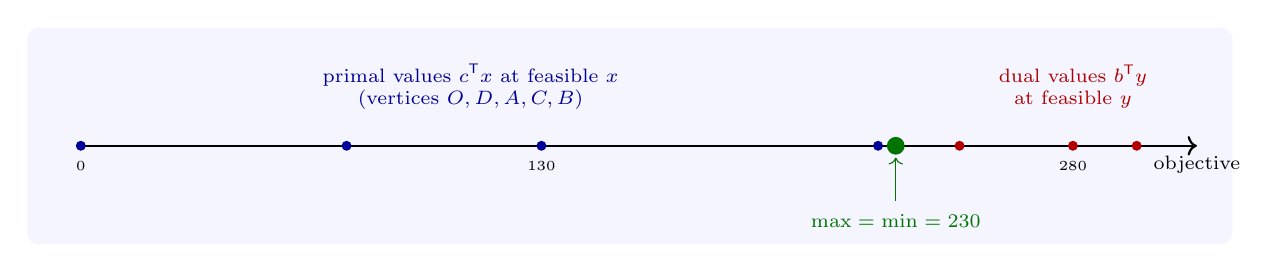
\begin{tikzpicture}[x=0.045cm,y=1cm]
\fill[blue!4,rounded corners=4pt] (-15,-1.25) rectangle (325,1.5);
\draw[->,thick] (0,0) -- (315,0) node[below,font=\scriptsize] {objective};
\foreach \v in {0,75,130,225,230} \fill[blue!60!black] (\v,0) circle (1.8pt);
\foreach \v in {248,280,298} \fill[red!70!black] (\v,0) circle (1.8pt);
\fill[green!45!black] (230,0) circle (3.2pt);
\node[font=\scriptsize,blue!60!black,align=center] at (110,0.75) {primal values $c^{\mathsf T}x$ at feasible $x$\\(vertices $O, D, A, C, B$)};
\node[font=\scriptsize,red!70!black,align=center] at (280,0.75) {dual values $b^{\mathsf T}y$\\at feasible $y$};
\draw[green!45!black,->] (230,-0.7) -- (230,-0.15);
\node[font=\scriptsize\bfseries,green!45!black] at (230,-0.95) {$\max = \min = 230$};
\foreach \v/\l in {0/0,130/130,280/280} \node[font=\tiny,below] at (\v,-0.08) {$\l$};
\end{tikzpicture}
\caption{Weak and strong duality for Example~\ref{ex:dualproductmix}. Every primal feasible value lies to the left of every dual feasible value; the dual values $248$, $280$ and $298$ shown come from the feasible prices $y = (2, \frac72, 0)$, $(0, 5, 0)$ and $(5, 3, 0)$. The two sets meet at the common optimum $230$.}
\label{fig:duality}
\end{figure}

\subsection{Complementary slackness}
\label{ssec:compslack}

\begin{thm}[Complementary slackness]
\label{thm:compslack}
Feasible $x$ for (P) and $y$ for (D) are both optimal if and only if
\[
y_i\bigl(b_i - (Ax)_i\bigr) = 0 \text{ for every } i, \qquad x_j\bigl((A^{\mathsf T}y)_j - c_j\bigr) = 0 \text{ for every } j .
\]
\end{thm}

\begin{proof}
In the proof of weak duality, $b^{\mathsf T}y - c^{\mathsf T}x = y^{\mathsf T}(b - Ax) + x^{\mathsf T}(A^{\mathsf T}y - c)$, a sum of non-negative terms. It is zero, which by strong duality is optimality, if and only if every term is zero.
\end{proof}

In words: a resource that is not fully used has price zero, and a resource with a positive price is fully used; a product that is made just breaks even at the dual prices, and a product that would lose money at those prices is not made. In Example~\ref{ex:dualproductmix} the third constraint has slack $3$ at the optimum,
so $y_3 = 0$, and both products are made, so both dual constraints are tight: $2y_1 + 2y_2 = 10$ and $y_1 + 4y_2 = 15$, which give $y = (\frac53, \frac{10}3, 0)$ without solving the dual. This is the usual way to recover dual solutions by hand, and to check that a proposed solution is optimal.

\subsection{Farkas' lemma}
\label{ssec:farkas}

Duality gives a short proof of the classical theorem of the alternative.

\begin{thm}[Farkas' lemma]
\label{thm:farkas}
Exactly one of the following has a solution: (a) $Ax \leq b$; (b) $y \geq 0$ with $A^{\mathsf T}y = 0$ and $b^{\mathsf T}y < 0$.
\end{thm}

\begin{proof}
Both cannot hold: $0 = (A^{\mathsf T}y)^{\mathsf T}x = y^{\mathsf T}Ax \leq y^{\mathsf T}b < 0$. Suppose (a) fails. The LP ``maximise $0$ subject to $Ax \leq b$'' (with $x$ free) is infeasible, so its dual ``minimise $b^{\mathsf T}y$ subject to $A^{\mathsf T}y = 0$, $y \geq 0$'' is either infeasible or unbounded. It is
feasible ($y = 0$), so it is unbounded, and some feasible $y$ has $b^{\mathsf T}y < 0$.
\end{proof}

A solution of (b) is a \textbf{certificate of infeasibility}: a non-negative combination of the constraints that reads $0 \leq$ (a negative number). Solvers return such certificates, and they are easy to check. For $x_1 + x_2 \leq 2$ and $x_1 + x_2 \geq 3$, the combination with weights $(\frac12, \frac12)$ of $x_1 + x_2 \leq 2$
and $-x_1 - x_2 \leq -3$ gives $0 \leq -\frac12$ (Software~\ref{sw:farkas}).

\subsection{The dual simplex method}
\label{ssec:dualsimplex}

The primal simplex method keeps $x_B \geq 0$ (primal feasibility) and works towards non-negative reduced costs (dual feasibility). The \textbf{dual simplex method} (Lemke, 1954) does the opposite: it keeps the reduced costs non-negative and works towards $x_B \geq 0$. An iteration chooses a row $r$ with
$x_{B(r)} < 0$ to leave, and among the columns with a negative entry in that row chooses the entering one by the \textbf{dual ratio test}
\[
j = \operatorname*{arg\,min}\Bigl\{\frac{\bar c_j}{|T_{rj}|} : T_{rj} < 0\Bigr\} ,
\]
which keeps every reduced cost non-negative after the pivot. If no entry of the row is negative, the row reads $\sum_jT_{rj}x_j = x_{B(r)} < 0$ with $T_{rj} \geq 0$, which no $x \geq 0$ satisfies, so the primal is infeasible. The objective value moves monotonically towards the optimum from the other side, and the method is the
simplex method applied to the dual, carried out on the primal tableau.

It is the natural method when a solved problem gains a constraint, as in the branch-and-bound and cutting-plane methods for integer programming: the old optimal basis stays dual feasible, the new constraint makes it primal infeasible, and a few dual pivots restore optimality. It is also the default of most modern solvers,
because it handles bounds and degeneracy well.

\begin{exa}
\label{ex:dualsimplex}
Minimise $20x_1 + 10x_2$ subject to $x_1 + 2x_2 \leq 40$, $3x_1 + x_2 \geq 30$, $4x_1 + 3x_2 \geq 60$. Multiplying the $\geq$ rows by $-1$ and adding slacks, the slack basis has $x_B = (40, -30, -60)$, primal infeasible, but reduced costs $(20, 10) \geq 0$, dual feasible. The most negative row, $-60$,
leaves; the dual ratios are $20/4 = 5$ and $10/3$, so $x_2$ enters. Then the second row, now $-10$, leaves and $x_1$ enters, giving the optimum $(6, 12)$ at cost $240$ in two pivots without any artificial variables (Software~\ref{sw:dualsimplex}).
\end{exa}

\subsection{Duality in software}
\label{ssec:software5}

\begin{software}[A primal--dual pair]
\label{sw:dual}
Example~\ref{ex:dualproductmix} and its dual solved separately, the multipliers that HiGHS returns with the primal solution, and the products in the complementary slackness conditions:
{\small\begin{verbatim}
>>> import numpy as np
>>> from scipy.optimize import linprog
>>> A = np.array([[2., 1], [2, 4], [-1, 1]]); b = np.array([26., 56, 5])
>>> c = np.array([10., 15])
>>> P = linprog(-c, A_ub=A, b_ub=b, method='highs')        # primal: max c x
>>> D = linprog(b, A_ub=-A.T, b_ub=-c, method='highs')     # dual: min b y
>>> P.x, -P.fun, D.x, D.fun                # A^T y >= c, y >= 0
(array([ 8., 10.]), 230.0, array([1.66666667, 3.33333333, 0.        ]), 230.0)
>>> -P.ineqlin.marginals                   # HiGHS's multipliers: the dual
array([1.66666667, 3.33333333, 0.        ])
>>> slack = b - A @ P.x; surplus = A.T @ D.x - c
>>> np.round(slack * D.x, 9) + 0, np.round(surplus * P.x, 9) + 0   # all 0
(array([0., 0., 0.]), array([0., 0.]))
\end{verbatim}}
\textbf{Reading the output.} The primal optimum $(8, 10)$ and the dual optimum $(\frac53, \frac{10}3, 0)$ have the same value $230$. HiGHS reports the dual solution as the \texttt{marginals} of the inequality constraints (with a minus sign, because it minimised $-Z$), so solving the dual separately is never necessary.
Every product $y_i \times \text{slack}_i$ and $x_j \times \text{surplus}_j$ is zero.

\textbf{MATLAB/Octave:} \texttt{[x, fval, flag, out, lambda] = linprog(...)}; the dual is \texttt{lambda.ineqlin}.
\end{software}

\begin{software}[The dual simplex method]
\label{sw:dualsimplex}
A dual simplex method on the tableau, in exact arithmetic, for Example~\ref{ex:dualsimplex}; each line shows the basis (columns $0, 1$ are $x_1, x_2$, $2, 3, 4$ the slacks), the right-hand sides and the objective value:
{\small\begin{verbatim}
>>> from fractions import Fraction as F
>>> def dual_simplex(T, basis):
...     """T: rows [A | b], last row [c | -z] with c >= 0 (dual feasible).
...     Pivots until b >= 0 (primal feasible), printing each basis."""
...     while True:
...         rhs = [str(T[i][-1]) for i in range(len(T) - 1)]
...         print(basis, rhs, -T[-1][-1])
...         r = min(range(len(T) - 1), key=lambda i: T[i][-1])
...         if T[r][-1] >= 0: return
...         cols = [j for j in range(len(T[0]) - 1) if T[r][j] < 0]
...         if not cols: raise ValueError('primal infeasible')
...         j = min(cols, key=lambda j: T[-1][j] / -T[r][j])   # ratio test
...         T[r] = [v / T[r][j] for v in T[r]]
...         for i in range(len(T)):
...             if i != r:
...                 T[i] = [a - T[i][j] * p for a, p in zip(T[i], T[r])]
...         basis[r] = j
...
>>> T = [[F(v) for v in row] for row in
...      [[1, 2, 1, 0, 0, 40],              # x1 + 2 x2 <= 40
...       [-3, -1, 0, 1, 0, -30],           # 3 x1 + x2 >= 30, times -1
...       [-4, -3, 0, 0, 1, -60],           # 4 x1 + 3 x2 >= 60, times -1
...       [20, 10, 0, 0, 0, 0]]]            # minimise 20 x1 + 10 x2
>>> dual_simplex(T, [2, 3, 4])             # start from the slack basis
[2, 3, 4] ['40', '-30', '-60'] 0
[2, 3, 1] ['0', '-10', '20'] 200
[2, 0, 1] ['10', '6', '12'] 240
\end{verbatim}}
\textbf{Reading the output.} The right-hand sides start at $(40, -30, -60)$ and become non-negative after two pivots. The objective rises from $0$ to $200$ to $240$: in the dual simplex method the value approaches the optimum from below for a minimisation, since each intermediate basis gives a feasible dual solution and
hence a lower bound.

\textbf{MATLAB/Octave:} the same row operations; \texttt{linprog} with \texttt{'dual-simplex'} uses this method.
\end{software}

\begin{software}[A certificate of infeasibility]
\label{sw:farkas}
For the infeasible system $x_1 + x_2 \leq 2$, $-x_1 - x_2 \leq -3$, a Farkas vector found by linear programming, normalised so that its entries sum to $1$:
{\small\begin{verbatim}
>>> A = np.array([[1., 1], [-1, -1]]); b = np.array([2., -3])  # x1 + x2 <= 2,
>>> far = linprog(b, A_eq=np.vstack([A.T, np.ones(2)]),        # x1 + x2 >= 3
...               b_eq=[0, 0, 1], method='highs')  # y >= 0, y A = 0, sum 1
>>> far.x, far.fun                         # y b < 0: a proof of infeasibility
(array([0.5, 0.5]), -0.5)
\end{verbatim}}
\textbf{Reading the output.} $y = (\frac12, \frac12)$ satisfies $A^{\mathsf T}y = 0$ with $b^{\mathsf T}y = -\frac12 < 0$: adding half of each constraint gives $0 \leq -\frac12$, an impossibility that proves the system has no solution.

\textbf{MATLAB/Octave:} the same \texttt{linprog} call with \texttt{Aeq = [A'; ones(1,2)]}.
\end{software}

\subsection{Practice Problems}

\begin{problem}
Write the dual of: minimise $3x_1 + 2x_2 + x_3$ subject to $x_1 + x_2 + x_3 \geq 6$, $2x_1 - x_2 = 1$, $x_1, x_3 \geq 0$, $x_2$ free.
\end{problem}

\begin{solution}
With dual variables $y_1 \geq 0$ for the $\geq$ row (in a minimisation) and $y_2$ free for the equation: maximise $6y_1 + y_2$ subject to $y_1 + 2y_2 \leq 3$ (from $x_1 \geq 0$), $y_1 - y_2 = 2$ (from $x_2$ free), $y_1 \leq 1$ (from $x_3 \geq 0$), $y_1 \geq 0$, $y_2$ free.
\end{solution}

\begin{problem}
Use complementary slackness to show that $x = (6, 12)$ is optimal for Example~\ref{ex:dualsimplex}, and find the dual solution.
\end{problem}

\begin{solution}
The dual is: maximise $-40w_1 + 30w_2 + 60w_3$ subject to $-w_1 + 3w_2 + 4w_3 \leq 20$, $-2w_1 + w_2 + 3w_3 \leq 10$, $w \geq 0$ (the first primal constraint written as $-x_1 - 2x_2 \geq -40$). At $x = (6, 12)$ the first constraint has slack $40 - 30 = 10$, so $w_1 = 0$; both $x_j > 0$, so both dual
constraints are tight: $3w_2 + 4w_3 = 20$, $w_2 + 3w_3 = 10$, giving $w_3 = 2$, $w_2 = 4$. These are non-negative, so $w$ is dual feasible, and $30\cdot 4 + 60\cdot 2 = 240$ equals the primal cost: both are optimal.
\end{solution}

\begin{problem}
\label{prob:bothinfeasible}
Show that the primal ``maximise $x_1 + x_2$ subject to $x_1 - x_2 \leq -1$, $-x_1 + x_2 \leq -1$, $x \geq 0$'' and its dual are both infeasible. What happens to the dual if the objective is $x_1 - x_2$ instead?
\end{problem}

\begin{solution}
Adding the primal constraints gives $0 \leq -2$, so the primal is infeasible. The dual is: minimise $-y_1 - y_2$ subject to $y_1 - y_2 \geq 1$, $-y_1 + y_2 \geq 1$, $y \geq 0$, and adding its constraints gives $0 \geq 2$: infeasible too. With the objective $x_1 - x_2$ the dual constraints become
$y_1 - y_2 \geq 1$ and $-y_1 + y_2 \geq -1$, which force $y_1 - y_2 = 1$ and are satisfied by $y = (1 + t, t)$ for every $t \geq 0$; the dual objective $-1 - 2t \to -\infty$, so the dual is unbounded, as it must be when the primal is infeasible and the dual feasible.
\end{solution}

\begin{problem}
In Example~\ref{ex:dualproductmix}, interpret $y_2 = \frac{10}3$ and predict the profit if the second resource rises from $56$ to $60$ units.
\end{problem}

\begin{solution}
$y_2$ is the value of one more unit of the second resource. If the basis stays optimal, the profit rises by $4 \times \frac{10}3 = 13.3$, to $243.3$. Check: with $2x_1 + x_2 = 26$ and $2x_1 + 4x_2 = 60$, $x_2 = \frac{34}3$, $x_1 = \frac{22}3$, feasible for the third constraint ($-\frac{22}3 + \frac{34}3 = 4 \leq 5$), and
$10\cdot\frac{22}3 + 15\cdot\frac{34}3 = \frac{730}3 = 243.3$. How far the resource can change before the basis changes is the subject of the next section.
\end{solution}

\begin{problem}
Use Farkas' lemma to show that the system $x_1 + 2x_2 \leq 1$, $-x_1 \leq -2$, $-x_2 \leq 0$ has no solution, by exhibiting a certificate.
\end{problem}

\begin{solution}
Take $y = (1, 1, 2)$: $A^{\mathsf T}y = (1 - 1 + 0, 2 + 0 - 2) = (0, 0)$, and $b^{\mathsf T}y = 1 - 2 + 0 = -1 < 0$. Indeed adding the first constraint, the second and twice the third gives $0 \leq -1$.
\end{solution}

\begin{problem}
Show that if (P) has a feasible solution and (D) has a feasible solution, then both have optimal solutions.
\end{problem}

\begin{solution}
By weak duality, the primal objective is bounded above by $b^{\mathsf T}y$ for the feasible $y$, so (P) is feasible and bounded. A feasible bounded LP has an optimal solution: the simplex method with Bland's rule terminates, and it cannot end with unboundedness, so it ends at an optimal BFS. By strong duality (D)
then has an optimal solution too.
\end{solution}

%======================================================================
\section{Sensitivity Analysis and Parametric Programming}
\label{sec:sensitivity}

The data of a real LP are estimates: prices change, capacities are uncertain, new products are proposed. A solution is of little use unless we also know how it depends on the data. \textbf{Sensitivity analysis} answers, from the final basis alone and without re-solving, questions such as: over what range of a
resource does the present plan stay optimal, and what is an extra unit worth; how far can a price move before the plan should change; is a new product worth making. \textbf{Parametric programming} follows the solution as a parameter varies over its whole range. Both rest on one observation: a basis $B$
is optimal exactly when it is \emph{primal feasible}, $B^{-1}b \geq 0$, and \emph{dual feasible}, all reduced costs of the right sign; $b$ enters only the first condition and $c$ only the second.

Throughout, the running example is Example~\ref{ex:graphical} (maximise $10x_1 + 15x_2$ with resources $b = (26, 56, 5)$), with optimal basis $\{s_3, x_1, x_2\}$, $x_B = (3, 8, 10)$, $Z = 230$, and shadow prices $y = (\frac53, \frac{10}3, 0)$, and
\[
B^{-1} = \begin{pmatrix} 1 & -\frac12 & 1 \\ \frac23 & -\frac16 & 0 \\ -\frac13 & \frac13 & 0 \end{pmatrix}
\]
from the final tableau of Example~\ref{ex:tableau} (rows for $s_3$, $x_1$, $x_2$).

\subsection{Changes in the right-hand side}
\label{ssec:rhsranging}

\begin{thm}[Right-hand-side ranging]
\label{thm:rhsranging}
If $b_i$ changes to $b_i + \delta$, the basis $B$ remains optimal if and only if $x_B + \delta B^{-1}e_i \geq 0$. On that interval of $\delta$ the optimal solution is $x_B + \delta B^{-1}e_i$ and the optimal value is $Z + \delta y_i$.
\end{thm}

\begin{proof}
The reduced costs do not involve $b$, so dual feasibility is unaffected, and $B$ is optimal if and only if the new basic solution $B^{-1}(b + \delta e_i)$ is non-negative. The value is $c_B^{\mathsf T}B^{-1}(b + \delta e_i) = Z + \delta y_i$.
\end{proof}

\begin{exa}
\label{ex:rhsranging}
For the second resource, $B^{-1}e_2 = (-\frac12, -\frac16, \frac13)$, so the conditions are $3 - \frac\delta2 \geq 0$, $8 - \frac\delta6 \geq 0$ and $10 + \frac\delta3 \geq 0$, that is $-30 \leq \delta \leq 6$: the basis stays optimal for $26 \leq b_2 \leq 62$, and over that range each extra unit is worth
$y_2 = \frac{10}3$. Likewise $23 \leq b_1 \leq 56$ with $y_1 = \frac53$, and $b_3 \geq 2$ with $y_3 = 0$ (Software~\ref{sw:ranging}). At the end $b_2 = 62$ the slack $s_3$ reaches $0$; beyond it the third constraint binds, the basis changes, and the second resource is no longer worth anything.
\end{exa}

The shadow price is thus a \emph{local} value. Outside the range it changes, and the way it changes is described by the following theorem, the geometric content of sensitivity analysis.

\begin{thm}
\label{thm:valuefunction}
For the maximisation (P), let $z^*(b)$ be the optimal value as a function of $b$, over the set of $b$ for which (P) is feasible, and suppose the dual feasible set $\{y \geq 0 : A^{\mathsf T}y \geq c\}$ is non-empty with vertices $y^1, \ldots, y^K$. Then
\[
z^*(b) = \min_kb^{\mathsf T}y^k ,
\]
a concave piecewise linear function of $b$, whose slope in the direction $e_i$ on each piece is the shadow price $y_i$ of the corresponding optimal basis.
\end{thm}

\begin{proof}
By strong duality $z^*(b)$ equals the dual optimum $\min\{b^{\mathsf T}y : A^{\mathsf T}y \geq c, y \geq 0\}$, which is finite where (P) is feasible and, by the fundamental theorem applied to the dual, is attained at a vertex. So it is the minimum of the finitely many linear functions $b \mapsto b^{\mathsf T}y^k$, which is concave
and piecewise linear.
\end{proof}

Concavity is \textbf{diminishing returns}: each additional unit of a resource is worth no more than the one before (Figure~\ref{fig:parametric}). The theorem also explains why shadow prices can be ambiguous at a breakpoint, where two pieces meet and the optimal basis is degenerate: there the left and right slopes differ,
and a solver reports one of them.

\begin{figure}[H]
\centering
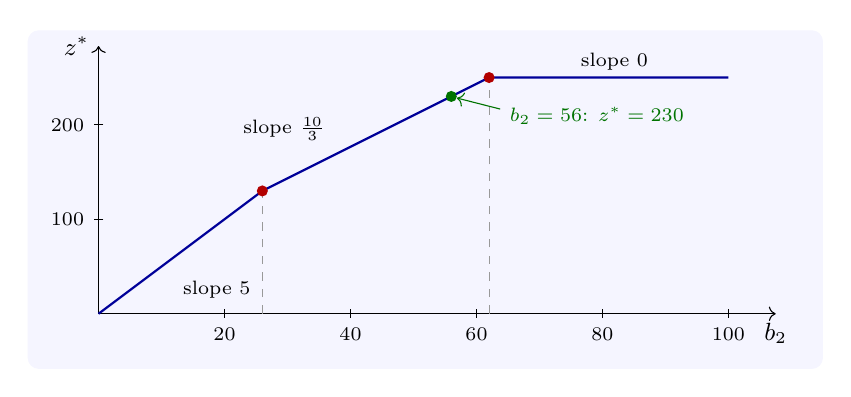
\begin{tikzpicture}[x=1cm,y=1cm]
\fill[blue!4,rounded corners=4pt] (-0.9,-0.7) rectangle (9.2,3.6);
\draw[->] (0,0) -- (8.6,0) node[below,font=\small] {$b_2$};
\draw[->] (0,0) -- (0,3.4) node[left,font=\small] {$z^*$};
\foreach \v in {20,40,60,80,100} \draw ({0.08*\v},0.06) -- ({0.08*\v},-0.06) node[below,font=\scriptsize] {$\v$};
\foreach \v in {100,200} \draw (0.06,{0.012*\v}) -- (-0.06,{0.012*\v}) node[left,font=\scriptsize] {$\v$};
\draw[blue!60!black,thick] (0.000,-0.000) -- (0.080,0.060) -- (0.160,0.120) -- (0.240,0.180) -- (0.320,0.240) -- (0.400,0.300) -- (0.480,0.360) -- (0.560,0.420) -- (0.640,0.480) -- (0.720,0.540) -- (0.800,0.600) -- (0.880,0.660) -- (0.960,0.720) -- (1.040,0.780) -- (1.120,0.840) -- (1.200,0.900) -- (1.280,0.960) -- (1.360,1.020) -- (1.440,1.080) -- (1.520,1.140) -- (1.600,1.200) -- (1.680,1.260) -- (1.760,1.320) -- (1.840,1.380) -- (1.920,1.440) -- (2.000,1.500) -- (2.080,1.560) -- (2.160,1.600) -- (2.240,1.640) -- (2.320,1.680) -- (2.400,1.720) -- (2.480,1.760) -- (2.560,1.800) -- (2.640,1.840) -- (2.720,1.880) -- (2.800,1.920) -- (2.880,1.960) -- (2.960,2.000) -- (3.040,2.040) -- (3.120,2.080) -- (3.200,2.120) -- (3.280,2.160) -- (3.360,2.200) -- (3.440,2.240) -- (3.520,2.280) -- (3.600,2.320) -- (3.680,2.360) -- (3.760,2.400) -- (3.840,2.440) -- (3.920,2.480) -- (4.000,2.520) -- (4.080,2.560) -- (4.160,2.600) -- (4.240,2.640) -- (4.320,2.680) -- (4.400,2.720) -- (4.480,2.760) -- (4.560,2.800) -- (4.640,2.840) -- (4.720,2.880) -- (4.800,2.920) -- (4.880,2.960) -- (4.960,3.000) -- (5.040,3.000) -- (5.120,3.000) -- (5.200,3.000) -- (5.280,3.000) -- (5.360,3.000) -- (5.440,3.000) -- (5.520,3.000) -- (5.600,3.000) -- (5.680,3.000) -- (5.760,3.000) -- (5.840,3.000) -- (5.920,3.000) -- (6.000,3.000) -- (6.080,3.000) -- (6.160,3.000) -- (6.240,3.000) -- (6.320,3.000) -- (6.400,3.000) -- (6.480,3.000) -- (6.560,3.000) -- (6.640,3.000) -- (6.720,3.000) -- (6.800,3.000) -- (6.880,3.000) -- (6.960,3.000) -- (7.040,3.000) -- (7.120,3.000) -- (7.200,3.000) -- (7.280,3.000) -- (7.360,3.000) -- (7.440,3.000) -- (7.520,3.000) -- (7.600,3.000) -- (7.680,3.000) -- (7.760,3.000) -- (7.840,3.000) -- (7.920,3.000) -- (8.000,3.000);
\draw[black!40,dashed] (2.08,0) -- (2.08,1.56); \draw[black!40,dashed] (4.96,0) -- (4.96,3.0);
\fill[red!70!black] (2.08,1.56) circle (2pt); \fill[red!70!black] (4.96,3.0) circle (2pt); \fill[green!45!black] (4.48,2.76) circle (2pt);
\node[font=\scriptsize,anchor=west] at (0.95,0.3) {slope $5$};
\node[font=\scriptsize,anchor=east] at (3.0,2.35) {slope $\frac{10}3$};
\node[font=\scriptsize,anchor=west] at (6.0,3.2) {slope $0$};
\node[font=\scriptsize,green!45!black,anchor=north west] at (5.1,2.75) {$b_2 = 56$: $z^* = 230$};\draw[green!45!black,->] (5.1,2.6) -- (4.55,2.74);
\end{tikzpicture}
\caption{The optimal profit of Example~\ref{ex:graphical} as a function of the second resource $b_2$, computed by solving the LP at $241$ values. It is concave and piecewise linear, with breakpoints at $b_2 = 26$ and $b_2 = 62$; the slopes $5$, $\frac{10}3$ and $0$ are the shadow prices of the three optimal bases met
along the way. The present value $b_2 = 56$ lies inside the middle range found by ranging.}
\label{fig:parametric}
\end{figure}

\subsection{Changes in the objective}
\label{ssec:costranging}

A change in $c$ leaves $x_B = B^{-1}b$ feasible and alters only the reduced costs $\bar c_j = c_j - c_B^{\mathsf T}B^{-1}A_j$ (for the maximisation, optimal while all $\bar c_j \leq 0$).
\begin{itemize}
\item If $c_j$ belongs to a \textbf{non-basic} variable, only $\bar c_j$ changes, and by the same amount: the basis stays optimal while $c_j$ rises by less than $-\bar c_j$. This is how much a product's profit must improve before it is worth making.
\item If $c_k$ belongs to a \textbf{basic} variable, $c_B$ changes, so every reduced cost changes, linearly in $c_k$; the range is the interval on which all of them keep their sign. The solution $x$ is unchanged on that range, and the value changes by $x_k$ per unit change in $c_k$.
\end{itemize}
For the running example the ranges are $7.5 \leq c_1 \leq 30$ and $5 \leq c_2 \leq 20$ (Software~\ref{sw:ranging}), the second agreeing with the graphical calculation of the problem at the end of the section on geometry. The analogue of Theorem~\ref{thm:valuefunction} is that the optimal value is a \emph{convex} piecewise linear function of $c$, the maximum of
$c^{\mathsf T}v$ over the vertices $v$ of the primal region.

Ranges hold for one coefficient at a time. For simultaneous changes the \textbf{$100\%$ rule} (Bradley, Hax and Magnanti) gives a sufficient condition: if each change is expressed as a fraction of the allowed change in its direction, the basis remains optimal when the fractions add up to at most $1$.

\subsection{New variables and new constraints}
\label{ssec:newvars}

\textbf{A new variable} $x_{n + 1}$ with column $a$ and profit $c_{n + 1}$ is priced out with the existing shadow prices: its reduced profit is $c_{n + 1} - y^{\mathsf T}a$. If this is $\leq 0$ the present plan stays optimal and the new activity is not worth starting; if it is positive, $x_{n + 1}$ enters the basis and the
primal simplex method continues from the old optimum. A product using one unit of each resource ($a = (1, 1, 1)$) is worth making in the running example only if its profit exceeds $y^{\mathsf T}a = \frac53 + \frac{10}3 + 0 = 5$, the value of the resources it would consume (Software~\ref{sw:newvar}).

\textbf{A new constraint} that the present optimum satisfies changes nothing. If it is violated, add it with its slack, express it in the current basis, and the tableau is dual feasible but primal infeasible: the dual simplex method of the section on duality restores optimality, usually in a few pivots.

\subsection{Parametric programming}
\label{ssec:parametric}

In \textbf{parametric programming} the data depend on a parameter $\theta$, for example $b(\theta) = b + \theta d$, and the solution is traced for all $\theta$. By Theorem~\ref{thm:rhsranging} the basis stays optimal on an interval of $\theta$; at its end a basic variable reaches zero, a dual simplex pivot changes the basis, and
the next interval begins. The optimal value is linear on each interval and concave overall, with slope $y^{\mathsf T}d$ on each piece. For $c(\theta) = c + \theta d$ the roles are exchanged: primal simplex pivots at the breakpoints, and a convex value function. Figure~\ref{fig:parametric} is the case $d = e_2$.

\subsection{Sensitivity in software}
\label{ssec:software6}

\begin{software}[Ranging]
\label{sw:ranging}
From the optimal basis $\{s_3, x_1, x_2\}$ of the running example: $x_B$ and $y$, the range of each $b_i$ from Theorem~\ref{thm:rhsranging}, and the range of each $c_j$ over which the reduced costs keep their sign, found on a fine grid:
{\small\begin{verbatim}
>>> import numpy as np
>>> from scipy.optimize import linprog
>>> A = np.array([[2., 1], [2, 4], [-1, 1]]); b = np.array([26., 56, 5])
>>> c = np.array([10., 15])
>>> Af = np.hstack([A, np.eye(3)]); cf = np.r_[c, 0, 0, 0]   # with slacks
>>> basis = [4, 0, 1]                      # s3, x1, x2: the optimal basis
>>> Binv = np.linalg.inv(Af[:, basis]); xB = Binv @ b
>>> y = cf[basis] @ Binv; xB, y          # basic values and shadow prices
(array([ 3.,  8., 10.]), array([1.66666667, 3.33333333, 0.        ]))
>>> for i in range(3):                     # right-hand-side ranges
...     col = Binv[:, i]; t = -xB / np.where(col == 0, np.nan, col)
...     lo = np.nanmax(np.where(col > 0, t, np.nan), initial=-np.inf)
...     hi = np.nanmin(np.where(col < 0, t, np.nan), initial=np.inf)
...     print(f"b{i+1}: {b[i] + lo:6.2f} to {b[i] + hi:6.2f}, y = {y[i]:.4f}")
...
b1:  23.00 to  56.00, y = 1.6667
b2:  26.00 to  62.00, y = 3.3333
b3:   2.00 to    inf, y = 0.0000
>>> def still_optimal(cc):           # all reduced costs <= 0 (maximising)
...     cfull = np.r_[cc, 0, 0, 0]
...     return np.all(cfull - (cfull[basis] @ Binv) @ Af <= 1e-9)
...
>>> grid = np.linspace(0, 60, 60001)       # cost ranges, on a fine grid
>>> for j in range(2):
...     trial = lambda t: np.where(np.arange(2) == j, t, c)
...     ok = [t for t in grid if still_optimal(trial(t))]
...     print(f"c{j+1}: {min(ok):.2f} to {max(ok):.2f}")
...
c1: 7.50 to 30.00
c2: 5.00 to 20.00
\end{verbatim}}
\textbf{Reading the output.} The ranges are $23 \leq b_1 \leq 56$, $26 \leq b_2 \leq 62$, $b_3 \geq 2$, and $7.5 \leq c_1 \leq 30$, $5 \leq c_2 \leq 20$. The third resource has price $0$ and can grow without limit, but cannot fall below $2$, where its slack of $3$ is used up.

\textbf{MATLAB/Octave:} \texttt{Binv = inv(Af(:, basis))} and the same ratio formulas.
\end{software}

\begin{software}[The value function]
\label{sw:valuefunction}
The optimal profit for $241$ values of $b_2$ from $0$ to $120$, its breakpoints, and the distinct slopes between them:
{\small\begin{verbatim}
>>> bs = np.linspace(0, 120, 241); z = []
>>> for b2 in bs:                          # parametric right-hand side b2
...     r = linprog(-c, A_ub=A, b_ub=[26, b2, 5], method='highs')
...     z.append(-r.fun)
...
>>> slopes = np.round(np.diff(z) / np.diff(bs), 4)
>>> breaks = [bs[k] for k in range(1, len(slopes))
...           if slopes[k] != slopes[k - 1]]
>>> breaks, sorted(set(slopes), reverse=True)
([26.0, 62.0], [5.0, 3.3333, 0.0])
\end{verbatim}}
\textbf{Reading the output.} The slope changes at $b_2 = 26$ and $b_2 = 62$, exactly the ends of the range found by ranging, and the slopes are $5$, $\frac{10}3$ and $0$, decreasing as Theorem~\ref{thm:valuefunction} requires. Below $26$ the constraints $2x_1 + 4x_2 \leq b_2$ and $-x_1 + x_2 \leq 5$ bind and an extra unit of
$b_2$ is worth $5$; above $62$ the second resource is in surplus.

\textbf{MATLAB/Octave:} a loop of \texttt{linprog} calls.
\end{software}

\begin{software}[A new product and a new constraint]
\label{sw:newvar}
Pricing a new product with column $(1, 1, 1)$ and profit $12$, then re-solving with it; and re-solving the original problem with the added constraint $x_1 \leq 6$:
{\small\begin{verbatim}
>>> a3, c3 = np.array([1., 1, 1]), 12.0    # a new product: price it out
>>> y @ a3, c3 - y @ a3                    # reduced profit > 0: worth making
(5.0, 7.0)
>>> r = linprog(-np.r_[c, c3], A_ub=np.c_[A, a3], b_ub=b, method='highs')
>>> r.x, -r.fun
(array([ 7., 10.,  2.]), 244.0)
>>> r = linprog(-c, A_ub=np.r_[A, [[1, 0]]], b_ub=np.r_[b, 6],
...             method='highs')            # a new constraint x1 <= 6
>>> r.x, -r.fun
(array([ 6., 11.]), 225.0)
\end{verbatim}}
\textbf{Reading the output.} The resources the new product uses are worth $5$, so a profit of $12$ gives a reduced profit of $7 > 0$: it should be made. The new optimum makes $7$, $10$ and $2$ units for a profit of $244$. The constraint $x_1 \leq 6$ cuts off the old optimum $(8, 10)$, and the new optimum is the vertex
$C(6, 11)$ with $Z = 225$: the restriction costs $5$.

\textbf{MATLAB/Octave:} \texttt{linprog} with the extra column or row.
\end{software}

\subsection{Practice Problems}

\begin{problem}
In the running example, find the range of $b_1$ by hand from $B^{-1}$, and the optimal solution when $b_1 = 30$.
\end{problem}

\begin{solution}
$B^{-1}e_1 = (1, \frac23, -\frac13)$, so the conditions are $3 + \delta \geq 0$, $8 + \frac23\delta \geq 0$, $10 - \frac13\delta \geq 0$: $-3 \leq \delta \leq 30$, that is $23 \leq b_1 \leq 56$. At $b_1 = 30$, $\delta = 4$: $s_3 = 7$, $x_1 = 8 + \frac83 = \frac{32}3$, $x_2 = 10 - \frac43 = \frac{26}3$, and
$Z = 230 + 4 \cdot \frac53 = 236.7$.
\end{solution}

\begin{problem}
Derive the range $7.5 \leq c_1 \leq 30$ from the reduced costs.
\end{problem}

\begin{solution}
With $c_B = (0, c_1, 15)$ for $(s_3, x_1, x_2)$, the multipliers are $y = c_B^{\mathsf T}B^{-1} = (\frac23c_1 - 5, -\frac16c_1 + 5, 0)$, and the reduced profits of $s_1$ and $s_2$ are $-y_1$ and $-y_2$. Optimality requires $y_1 \geq 0$ and $y_2 \geq 0$: $c_1 \geq 7.5$ and $c_1 \leq 30$. At $c_1 = 10$ these give
$y = (\frac53, \frac{10}3, 0)$.
\end{solution}

\begin{problem}
A new product needs $3$, $1$ and $0$ units of the three resources. What profit per unit must it earn to be worth making?
\end{problem}

\begin{solution}
It is worth making if its profit exceeds $y^{\mathsf T}a = 3\cdot\frac53 + 1\cdot\frac{10}3 + 0 = \frac{25}3 = 8.33$.
\end{solution}

\begin{problem}
Using the 100\% rule, decide whether the basis stays optimal if $b_1$ rises by $10$ and $b_2$ falls by $15$ at the same time.
\end{problem}

\begin{solution}
The allowed increase of $b_1$ is $30$ and the allowed decrease of $b_2$ is $30$. The fractions are $\frac{10}{30} + \frac{15}{30} = \frac56 \leq 1$, so the basis remains optimal. Check:
\[
x_B = (3, 8, 10) + 10\bigl(1, \tfrac23, -\tfrac13\bigr) - 15\bigl(-\tfrac12, -\tfrac16, \tfrac13\bigr) = (20.5, 17.17, 1.67) \geq 0 .
\]
\end{solution}

\begin{problem}
Explain why the optimal value is a convex function of the cost vector $c$, for a fixed feasible region.
\end{problem}

\begin{solution}
For a bounded feasible region with vertices $v^1, \ldots, v^K$, the optimal value of the maximisation is $\max_kc^{\mathsf T}v^k$, a maximum of linear functions of $c$, which is convex. Economically, if prices can vary, being able to re-optimise is worth more the more they vary.
\end{solution}

\begin{problem}
In the running example the third resource has slack $3$ and price $0$. A consultant proposes buying $10$ more units of it at Rs.~1 each. Should the firm accept?
\end{problem}

\begin{solution}
No. Its shadow price is $0$ for all $b_3 \geq 2$, so extra units add no profit: the firm would pay Rs.~10 for nothing. The third resource is not a bottleneck; the first two are, worth $\frac53$ and $\frac{10}3$ per unit within their ranges.
\end{solution}

%SECTIONS

\section*{References}
\addcontentsline{toc}{section}{References}
\sloppy

\subhead{Principal texts}
\begin{enumerate}
\item Sharma, J. K. (2012), \emph{Operations Research: Problems and Solutions} (3rd ed.), New Delhi, Macmillan.
\item Hillier, F. S., and Lieberman, G. J. (2015), \emph{Introduction to Operations Research} (10th ed.), New York, McGraw-Hill.
\item Bertsimas, D., and Tsitsiklis, J. N. (1997), \emph{Introduction to Linear Optimization}, Belmont, Athena Scientific.
\end{enumerate}

\subhead{Recommended texts}
\begin{enumerate}
\item Chv\'atal, V. (1983), \emph{Linear Programming}, New York, W. H. Freeman.
\item Taha, H. A. (2017), \emph{Operations Research: An Introduction} (10th ed.), Harlow, Pearson.
\item Winston, W. L. (2004), \emph{Operations Research: Applications and Algorithms} (4th ed.), Belmont, Brooks/Cole.
\end{enumerate}

\subhead{Software}
\begin{enumerate}
\item Harris, C. R., et al. (2020), Array programming with NumPy, \emph{Nature}, 585, 357--362.
\item Virtanen, P., et al. (2020), SciPy 1.0: fundamental algorithms for scientific computing in Python, \emph{Nature Methods}, 17, 261--272.
\item Huangfu, Q., and Hall, J. A. J. (2018), Parallelizing the dual revised simplex method, \emph{Mathematical Programming Computation}, 10, 119--142.
\end{enumerate}

\subhead{Further reading}
\begin{enumerate}
\item Beale, E. M. L. (1955), Cycling in the dual simplex algorithm, \emph{Naval Research Logistics Quarterly}, 2, 269--275.
\item Blackett, P. M. S. (1962), \emph{Studies of War: Nuclear and Conventional}, Edinburgh, Oliver and Boyd.
\item Bland, R. G. (1977), New finite pivoting rules for the simplex method, \emph{Mathematics of Operations Research}, 2, 103--107.
\item Bradley, S. P., Hax, A. C., and Magnanti, T. L. (1977), \emph{Applied Mathematical Programming}, Reading, Addison-Wesley.
\item Charnes, A. (1952), Optimality and degeneracy in linear programming, \emph{Econometrica}, 20, 160--170.
\item Charnes, A., Cooper, W. W., and Ferguson, R. O. (1955), Optimal estimation of executive compensation by linear programming, \emph{Management Science}, 1, 138--151.
\item Dantzig, G. B. (1951), Maximization of a linear function of variables subject to linear inequalities, in T. C. Koopmans (ed.), \emph{Activity Analysis of Production and Allocation}, New York, Wiley, 339--347.
\item Dantzig, G. B. (1955), Upper bounds, secondary constraints, and block triangularity in linear programming, \emph{Econometrica}, 23, 174--183.
\item Dantzig, G. B., and Orchard-Hays, W. (1954), The product form for the inverse in the simplex method, \emph{Mathematical Tables and Other Aids to Computation}, 8, 64--67.
\item Farkas, J. (1902), Theorie der einfachen Ungleichungen, \emph{Journal f\"ur die reine und angewandte Mathematik}, 124, 1--27.
\item Forrest, J. J. H., and Tomlin, J. A. (1972), Updated triangular factors of the basis to maintain sparsity in the product form simplex method, \emph{Mathematical Programming}, 2, 263--278.
\item Gal, T., and Greenberg, H. J. (eds.) (1997), \emph{Advances in Sensitivity Analysis and Parametric Programming}, Boston, Kluwer.
\item Gale, D., Kuhn, H. W., and Tucker, A. W. (1951), Linear programming and the theory of games, in T. C. Koopmans (ed.), \emph{Activity Analysis of Production and Allocation}, New York, Wiley, 317--329.
\item Gass, S. I., and Saaty, T. L. (1955), The computational algorithm for the parametric objective function, \emph{Naval Research Logistics Quarterly}, 2, 39--45.
\item Goldfarb, D., and Reid, J. K. (1977), A practicable steepest-edge simplex algorithm, \emph{Mathematical Programming}, 12, 361--371.
\item Harris, P. M. J. (1973), Pivot selection methods of the Devex LP code, \emph{Mathematical Programming}, 5, 1--28.
\item Kantorovich, L. V. (1939), \emph{Mathematical Methods of Organizing and Planning Production} (in Russian), Leningrad State University; English translation (1960), \emph{Management Science}, 6, 366--422.
\item Karmarkar, N. (1984), A new polynomial-time algorithm for linear programming, \emph{Combinatorica}, 4, 373--395.
\item Khachiyan, L. G. (1979), A polynomial algorithm in linear programming, \emph{Soviet Mathematics Doklady}, 20, 191--194.
\item Klee, V., and Minty, G. J. (1972), How good is the simplex algorithm?, in O. Shisha (ed.), \emph{Inequalities III}, New York, Academic Press, 159--175.
\item Koopmans, T. C. (ed.) (1951), \emph{Activity Analysis of Production and Allocation}, New York, Wiley.
\item Lemke, C. E. (1954), The dual method of solving the linear programming problem, \emph{Naval Research Logistics Quarterly}, 1, 36--47.
\item Minkowski, H. (1896), \emph{Geometrie der Zahlen}, Leipzig, Teubner.
\item von Neumann, J. (1947), Discussion of a maximum problem, unpublished manuscript, in A. H. Taub (ed.), \emph{John von Neumann: Collected Works}, Vol.~VI (1963), Oxford, Pergamon, 89--95.
\item Spielman, D. A., and Teng, S.-H. (2004), Smoothed analysis of algorithms: why the simplex algorithm usually takes polynomial time, \emph{Journal of the ACM}, 51, 385--463.
\item Stigler, G. J. (1945), The cost of subsistence, \emph{Journal of Farm Economics}, 27, 303--314.
\item Weyl, H. (1935), Elementare Theorie der konvexen Polyeder, \emph{Commentarii Mathematici Helvetici}, 7, 290--306.
\end{enumerate}

\end{document}
